\lab{Applications}{Anisotropic Diffusion}{Anisotropic Diffusion}
\label{lab:AnisotropicDiffusion}

\objective{Demonstrate the use of finite difference schemes in image analysis.}

We will now look into one of the many applications of Finite Difference Methods.
It is often useful in image processing to remove extra static from an image.
This is most easy done by simply blurring the image, but this has the unfortunate consequence of also blurring the boundary lines between distinct elements of the image.
This blurring can be done by treating the image as a rectangular domain where we are applying the diffusion equation:
$$u_t = b \Delta u$$
where $b$ is some diffusion constant.
A more general form of the diffusion equation in two dimensions is:
$$u_t = div \left( c(x,y,t) \nabla u \right)$$
where $c$ is a function representing the diffusion coefficient at each given point and time.
Note that $div$ is the divergence operator and $\nabla$ is the gradient.
If we want to blur a picture uniformly, we can allow $c$ to be constant, but we are often interested in \textit{preserving the edges} of components of the image.
$c$ can be used to control how much diffusion is allowed at each point, so we would like to modify it so that it minimizes diffusion across edges in the image.
If we can limit diffusion near the boundaries of different elements of the image, we will be able to allow smaller details of the image to blur away while maintaining the overall form of the image.
This is especially useful for denoising low quality images. 
This approach was first introduced by Perona and Malik in 1987.
It is known as Anisotropic Diffusion or Perona-Malik Diffusion.

Suppose we have some estimate $E$ of the rate of change at a given point in an image.
This means that $E$ will be large at boundaries in the image and small elsewhere.
We will then let $c(x,y,t) = g(E(x,y,t))$ where $g$ is some function such that $g(0)=1$ and $\displaystyle{\lim_{x \to \infty} g(x) = 0}$. 
The idea here is that $c$ will be small where $E$ is large, so there will be little diffusion near the boundaries of different portions of the image.

We will implement this idea of limiting diffusion at edges in the following way:
The following finite difference scheme is consistent with the Laplace Operator:
$$\Delta u = u_{xx}+u_{yy} \approx \frac{v_{l-1,m}^n - 2 v_{l,m}^n + v_{l+1,m}^n}{(\Delta x)^2} + \frac{v_{l,m-1}-2 v_{l,m}^n + v_{l,m+1}^n}{(\Delta y)^2}$$
Since we are working with images, we may say, without loss of generality, that the distance between pixels is always one, so $\Delta x = \Delta y = 1$. Rearranging the terms we have:
$$ \Delta u \approx (v_{l-1,m}^n - v_{l,m}) + (v_{l+1,m}^n - v_{l,m}) + (v_{l,m-1} - v_{l,m}) + (v_{l,m+1} - v_{l,m})$$. 

Again, since we are working with images and not some time based problem, we may say, without loss of generality, that $\Delta t = 1$, so we will have the following finite difference scheme:
$$v_{l,m}^{n+1} = v_{l,m}^n + (v_{l-1,m}^n - v_{l,m}) + (v_{l+1,m}^n - v_{l,m}) + (v_{l,m-1} - v_{l,m}) + (v_{l,m+1} - v_{l,m})$$.
We will now limit the diffusion near the edges of objects by making the following modification:
\begin{equation*}
\begin{split}
v_{l,m}^{n+1} =& v_{l,m}^n + \lambda (g(|v_{l-1,m}^n - v_{l,m}|)(v_{l-1,m}^n - v_{l,m}) + g(|v_{l+1,m}^n - v_{l,m}|)(v_{l+1,m}^n - v_{l,m}) \\
 &+ g(|v_{l,m-1} - v_{l,m}|)(v_{l,m-1} - v_{l,m}) + g(|v_{l,m+1} - v_{l,m}|)(v_{l,m+1} - v_{l,m}))
\end{split}
\end{equation*}

Where $\lambda \leq \frac{1}{4}$ for stability.

In this way, we allow each term to be affected most by the terms that are already the most simlar to it, so less diffusion will happen anywhere where there is a sharp difference between pixels.

Two good examples of commonly used functions for $g$ are $g(x) = e^{-\left(\frac{x}{\sigma}\right)^2}$ and $g(x) = \frac{1}{1+\left(\frac{x}{\sigma}\right)^2}$. 
In both cases, $\sigma$ is a parameter which allows us to control how sharply we decrease diffusion across boundaries.
Larger $\sigma$ values allow more diffusion across boundaries.
Also note that in both cases, $g(0) = 1$ and $\displaystyle{\lim_{x\to \infty} g(x) = 0}$.

It is worth noting that this particular difference scheme is \textit{not} an accurate finite difference scheme for the version of the diffusion equation we discussed before, but it \textit{does} accomplish the same thing in the same way.

For all of the examples here we have read in the image using the \li{scipy.misc.imread} function, and normalized it so that the colors are represented as floating point values between 0 and 1.

\newpage
\vfill
\begin{figure}[ht]
\begin{minipage}[b]{0.45\linewidth}
\centering
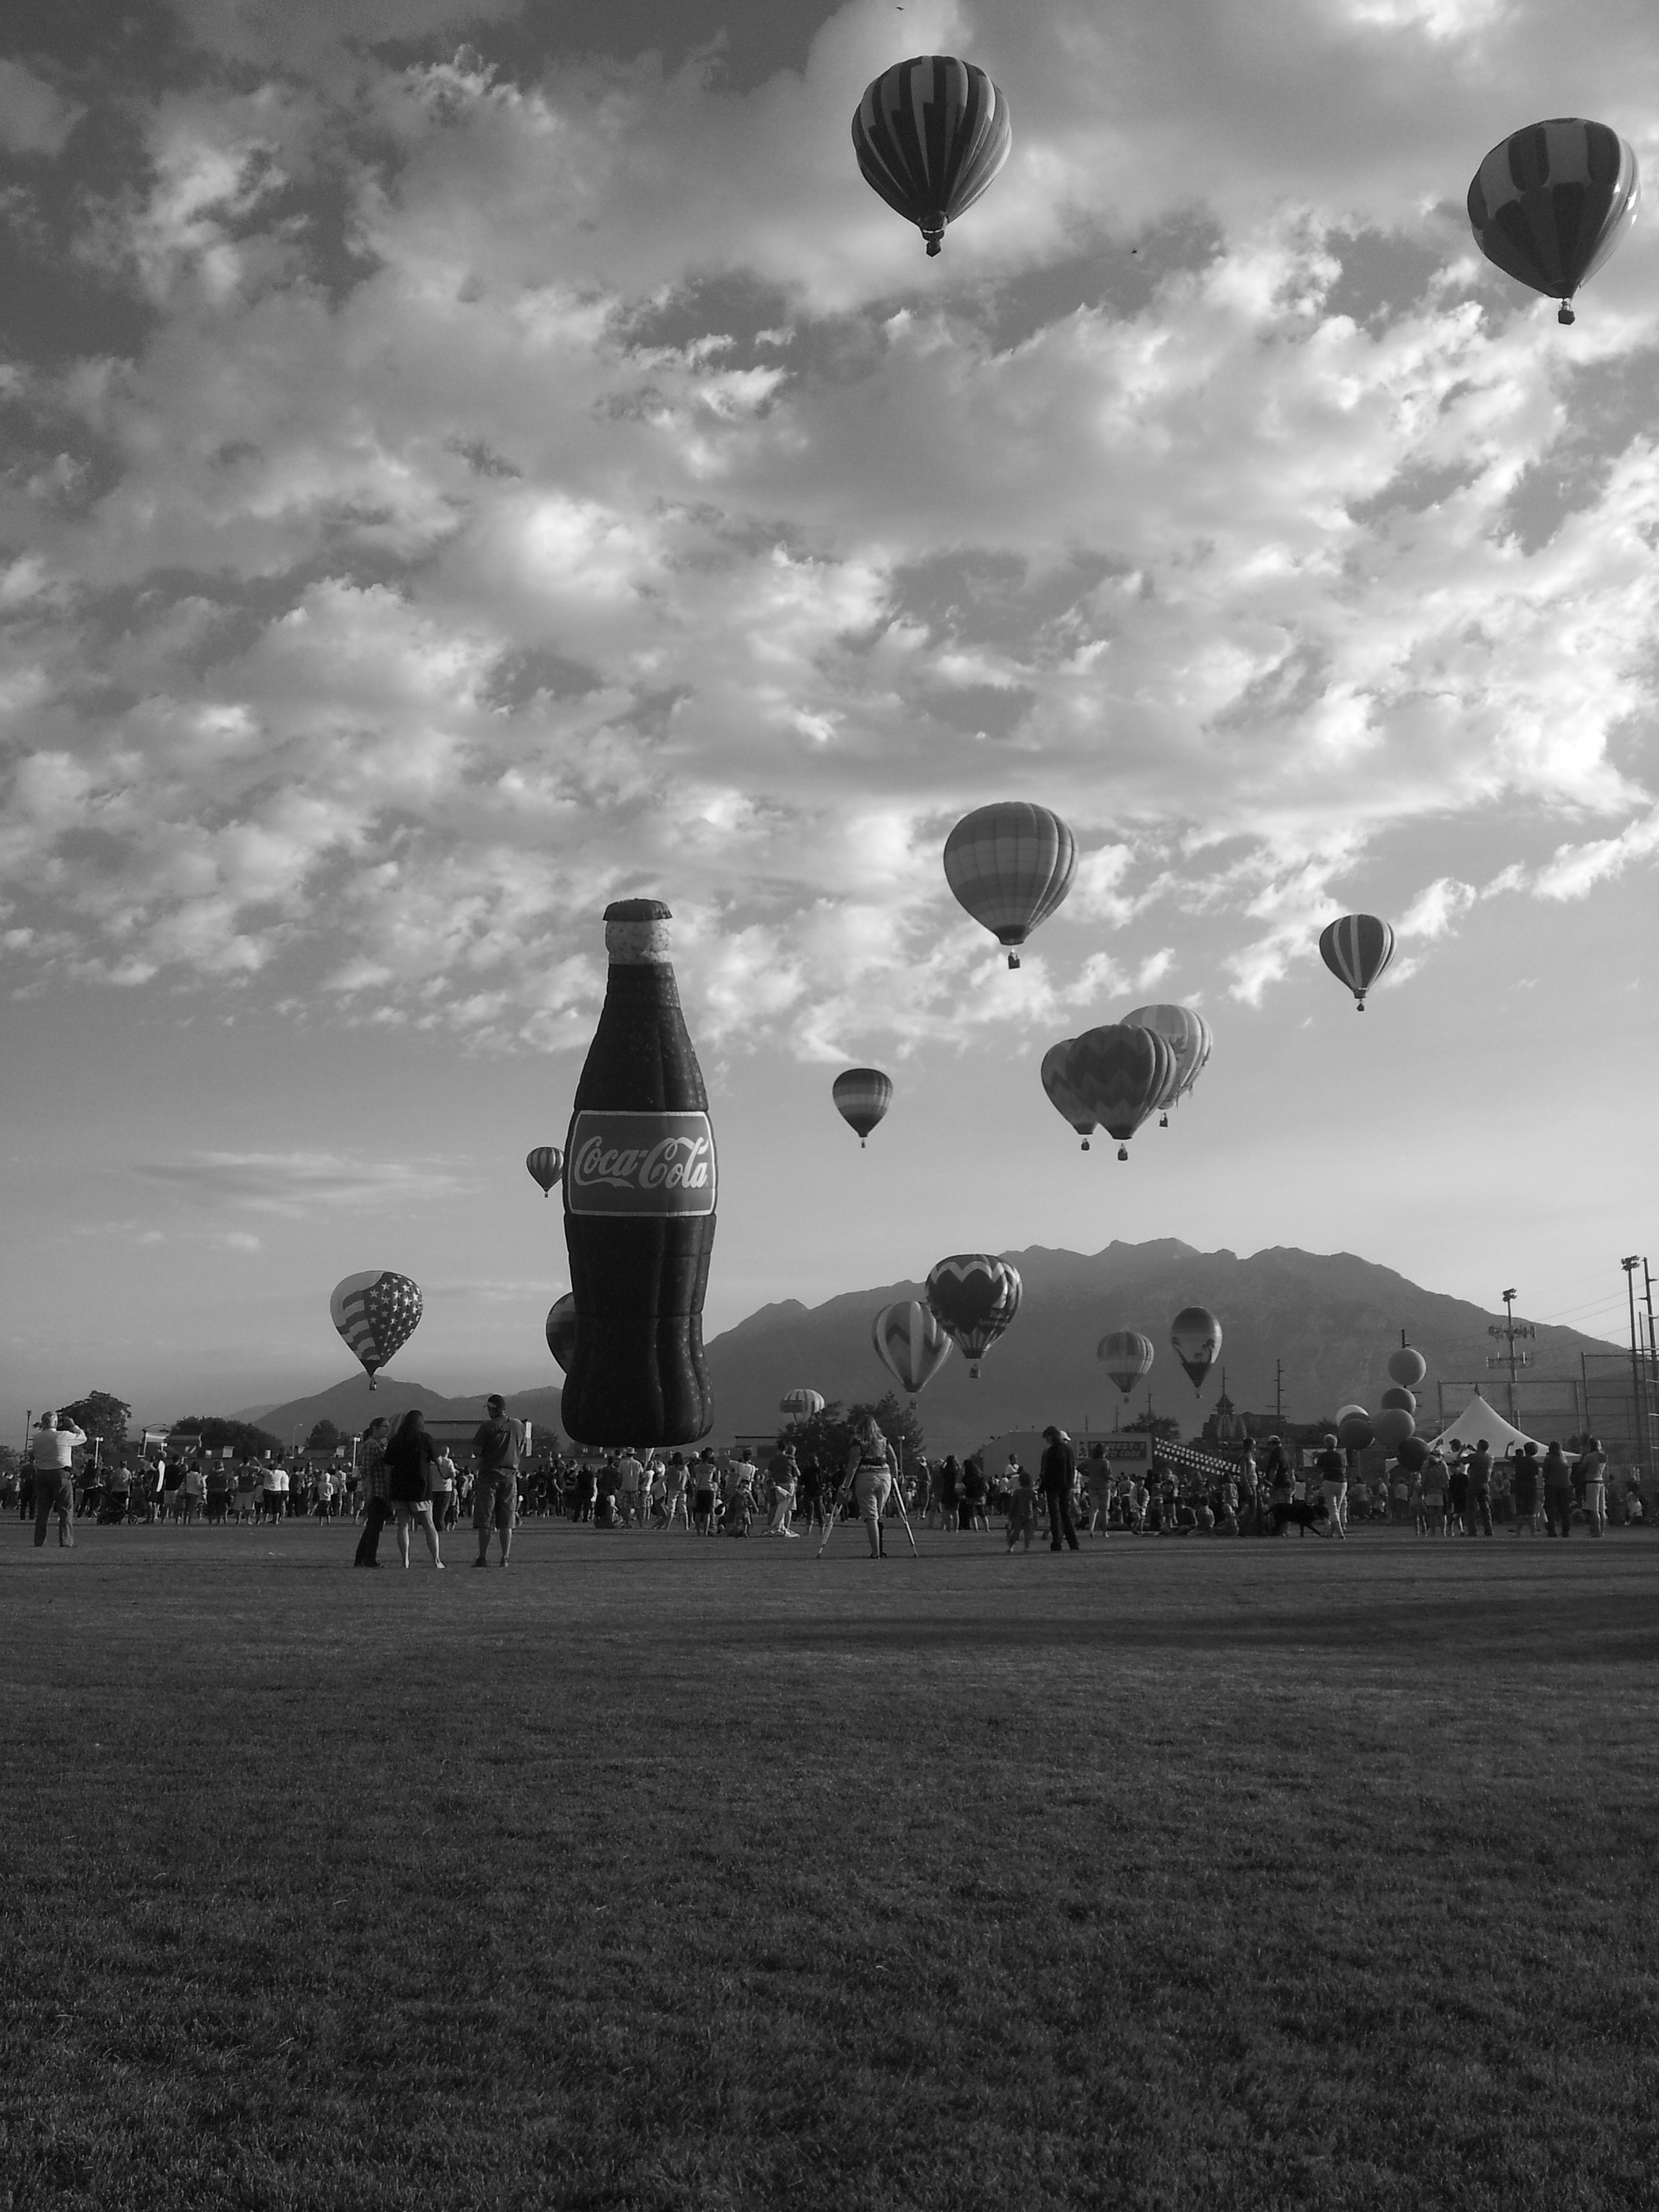
\includegraphics[width=\textwidth]{baloonbw}
\caption*{original image}
\end{minipage}
\hspace{0.5cm}
\begin{minipage}[b]{0.45\linewidth}
\centering
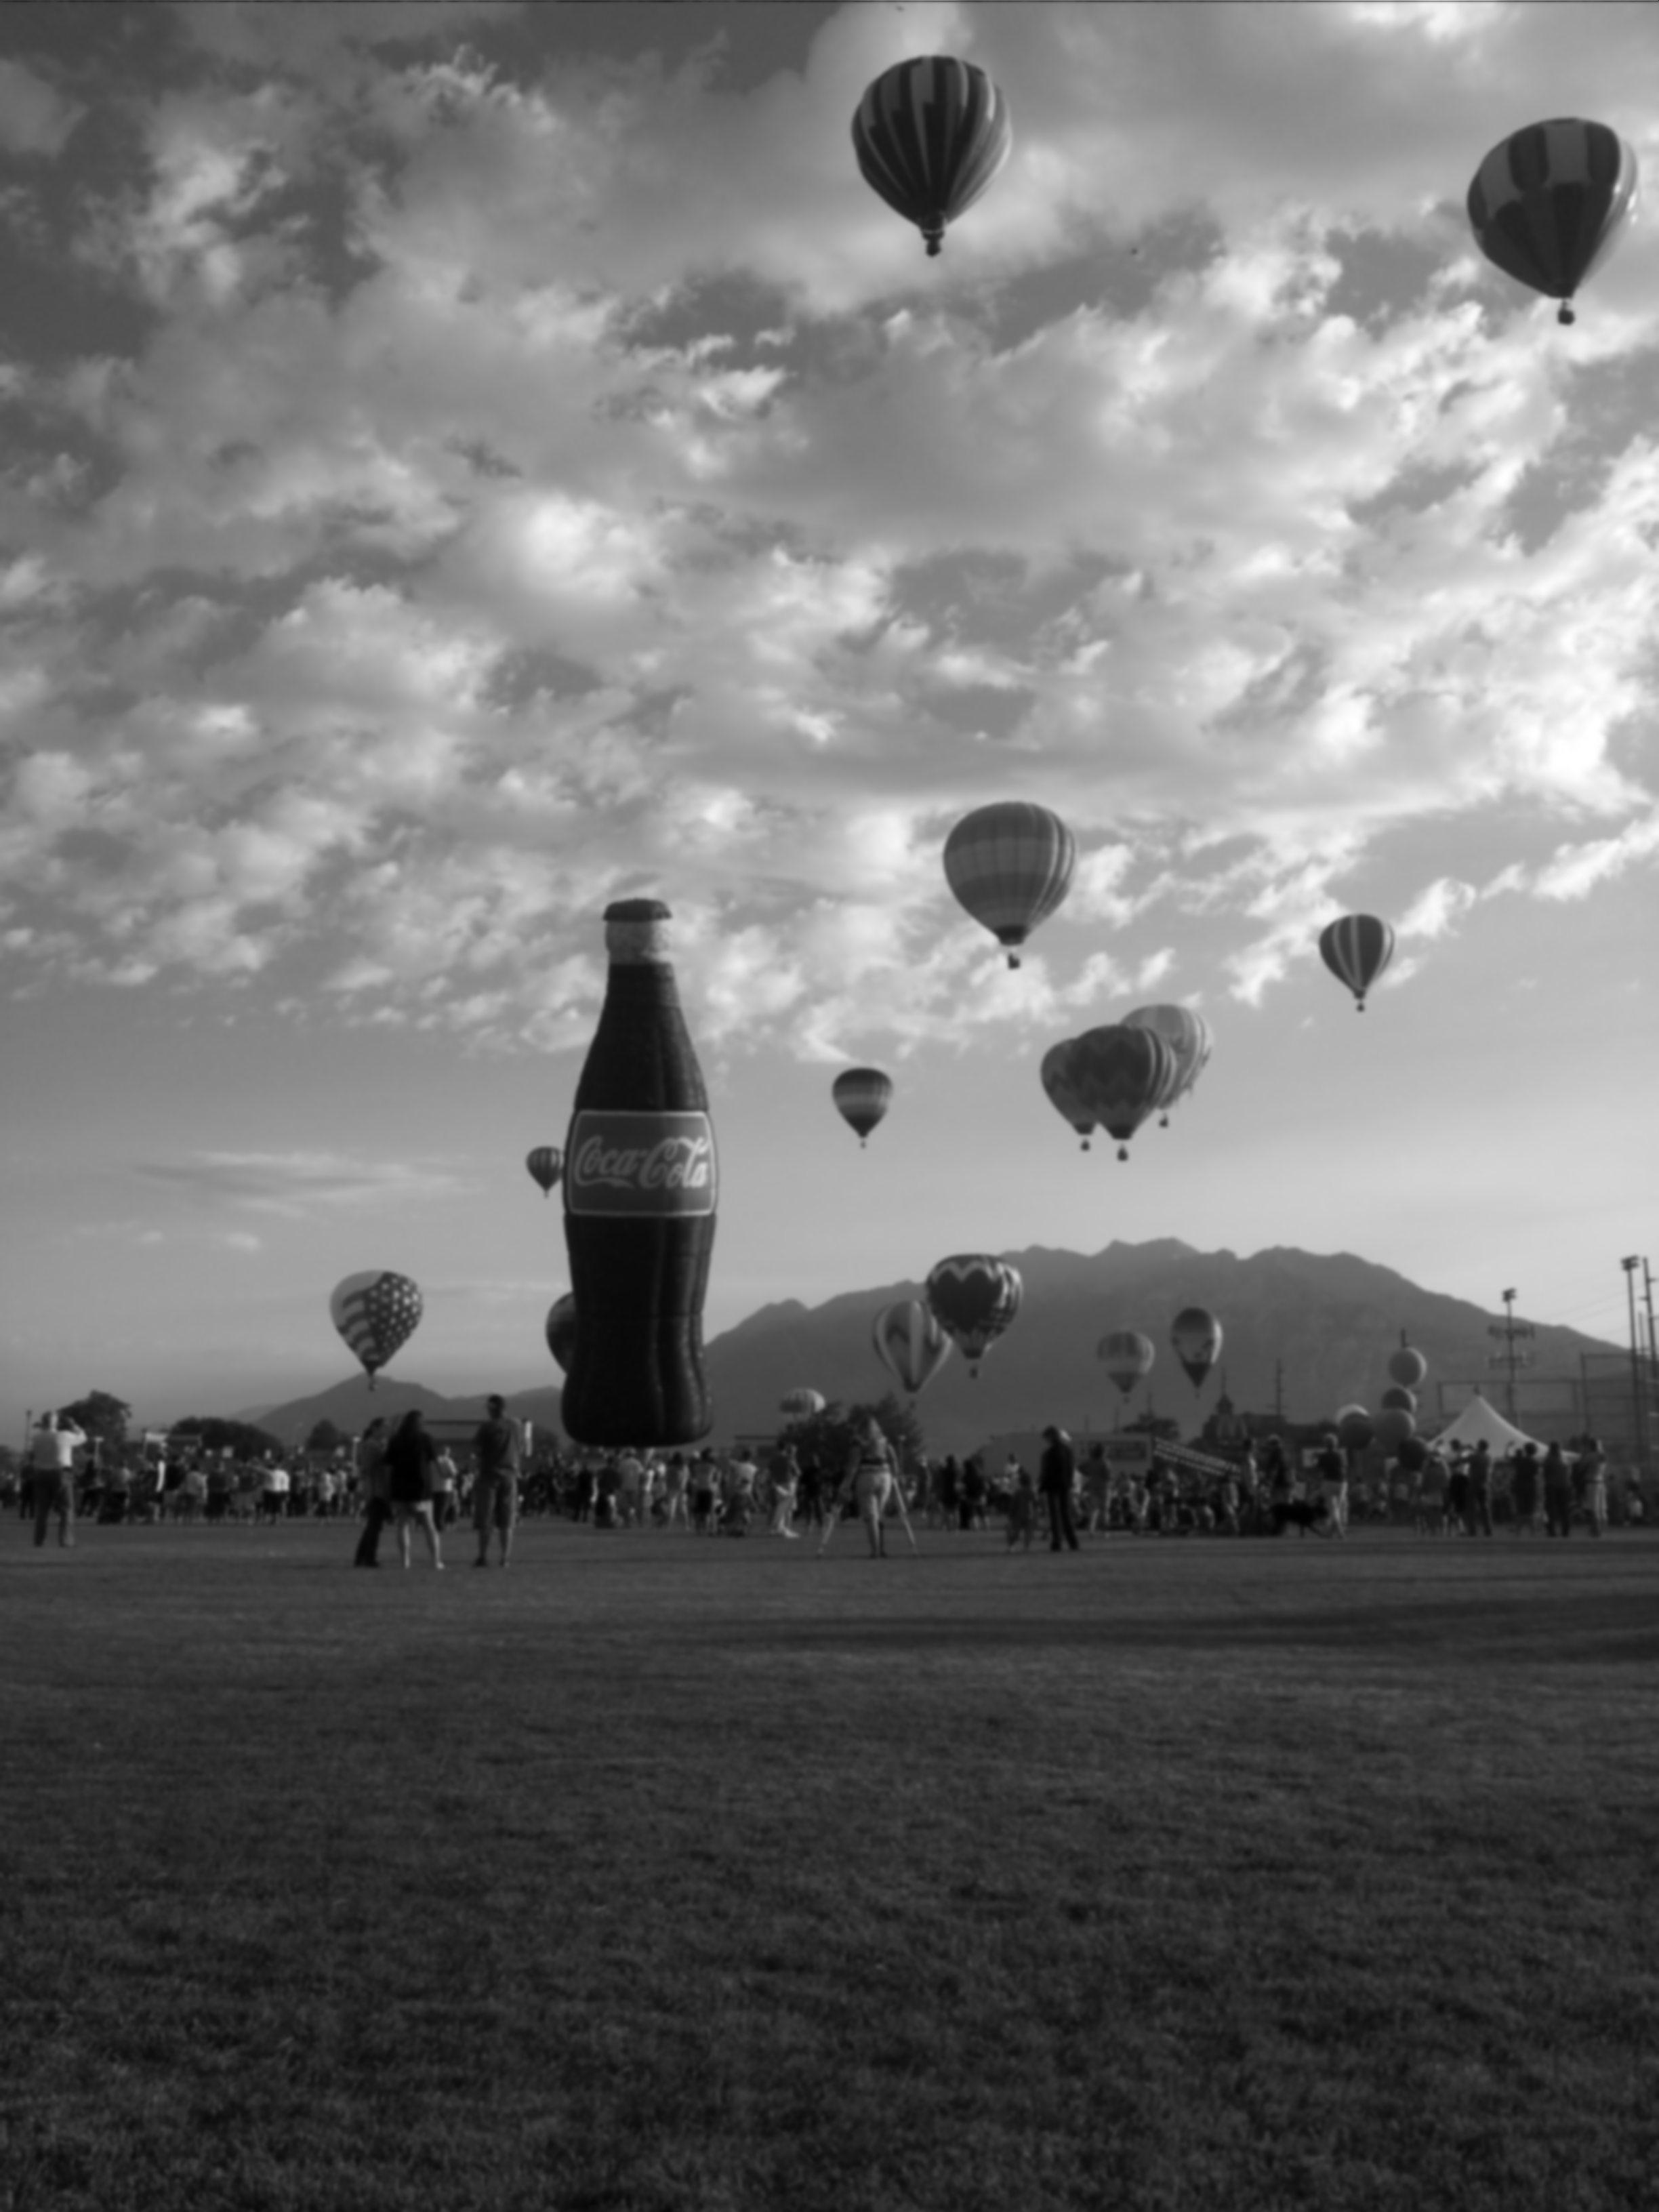
\includegraphics[width=\textwidth]{baloon20}
\caption*{after 20 iterations with $\sigma = .7$ and $\lambda = .2$}
\end{minipage}
\begin{minipage}[b]{0.45\linewidth}
\centering
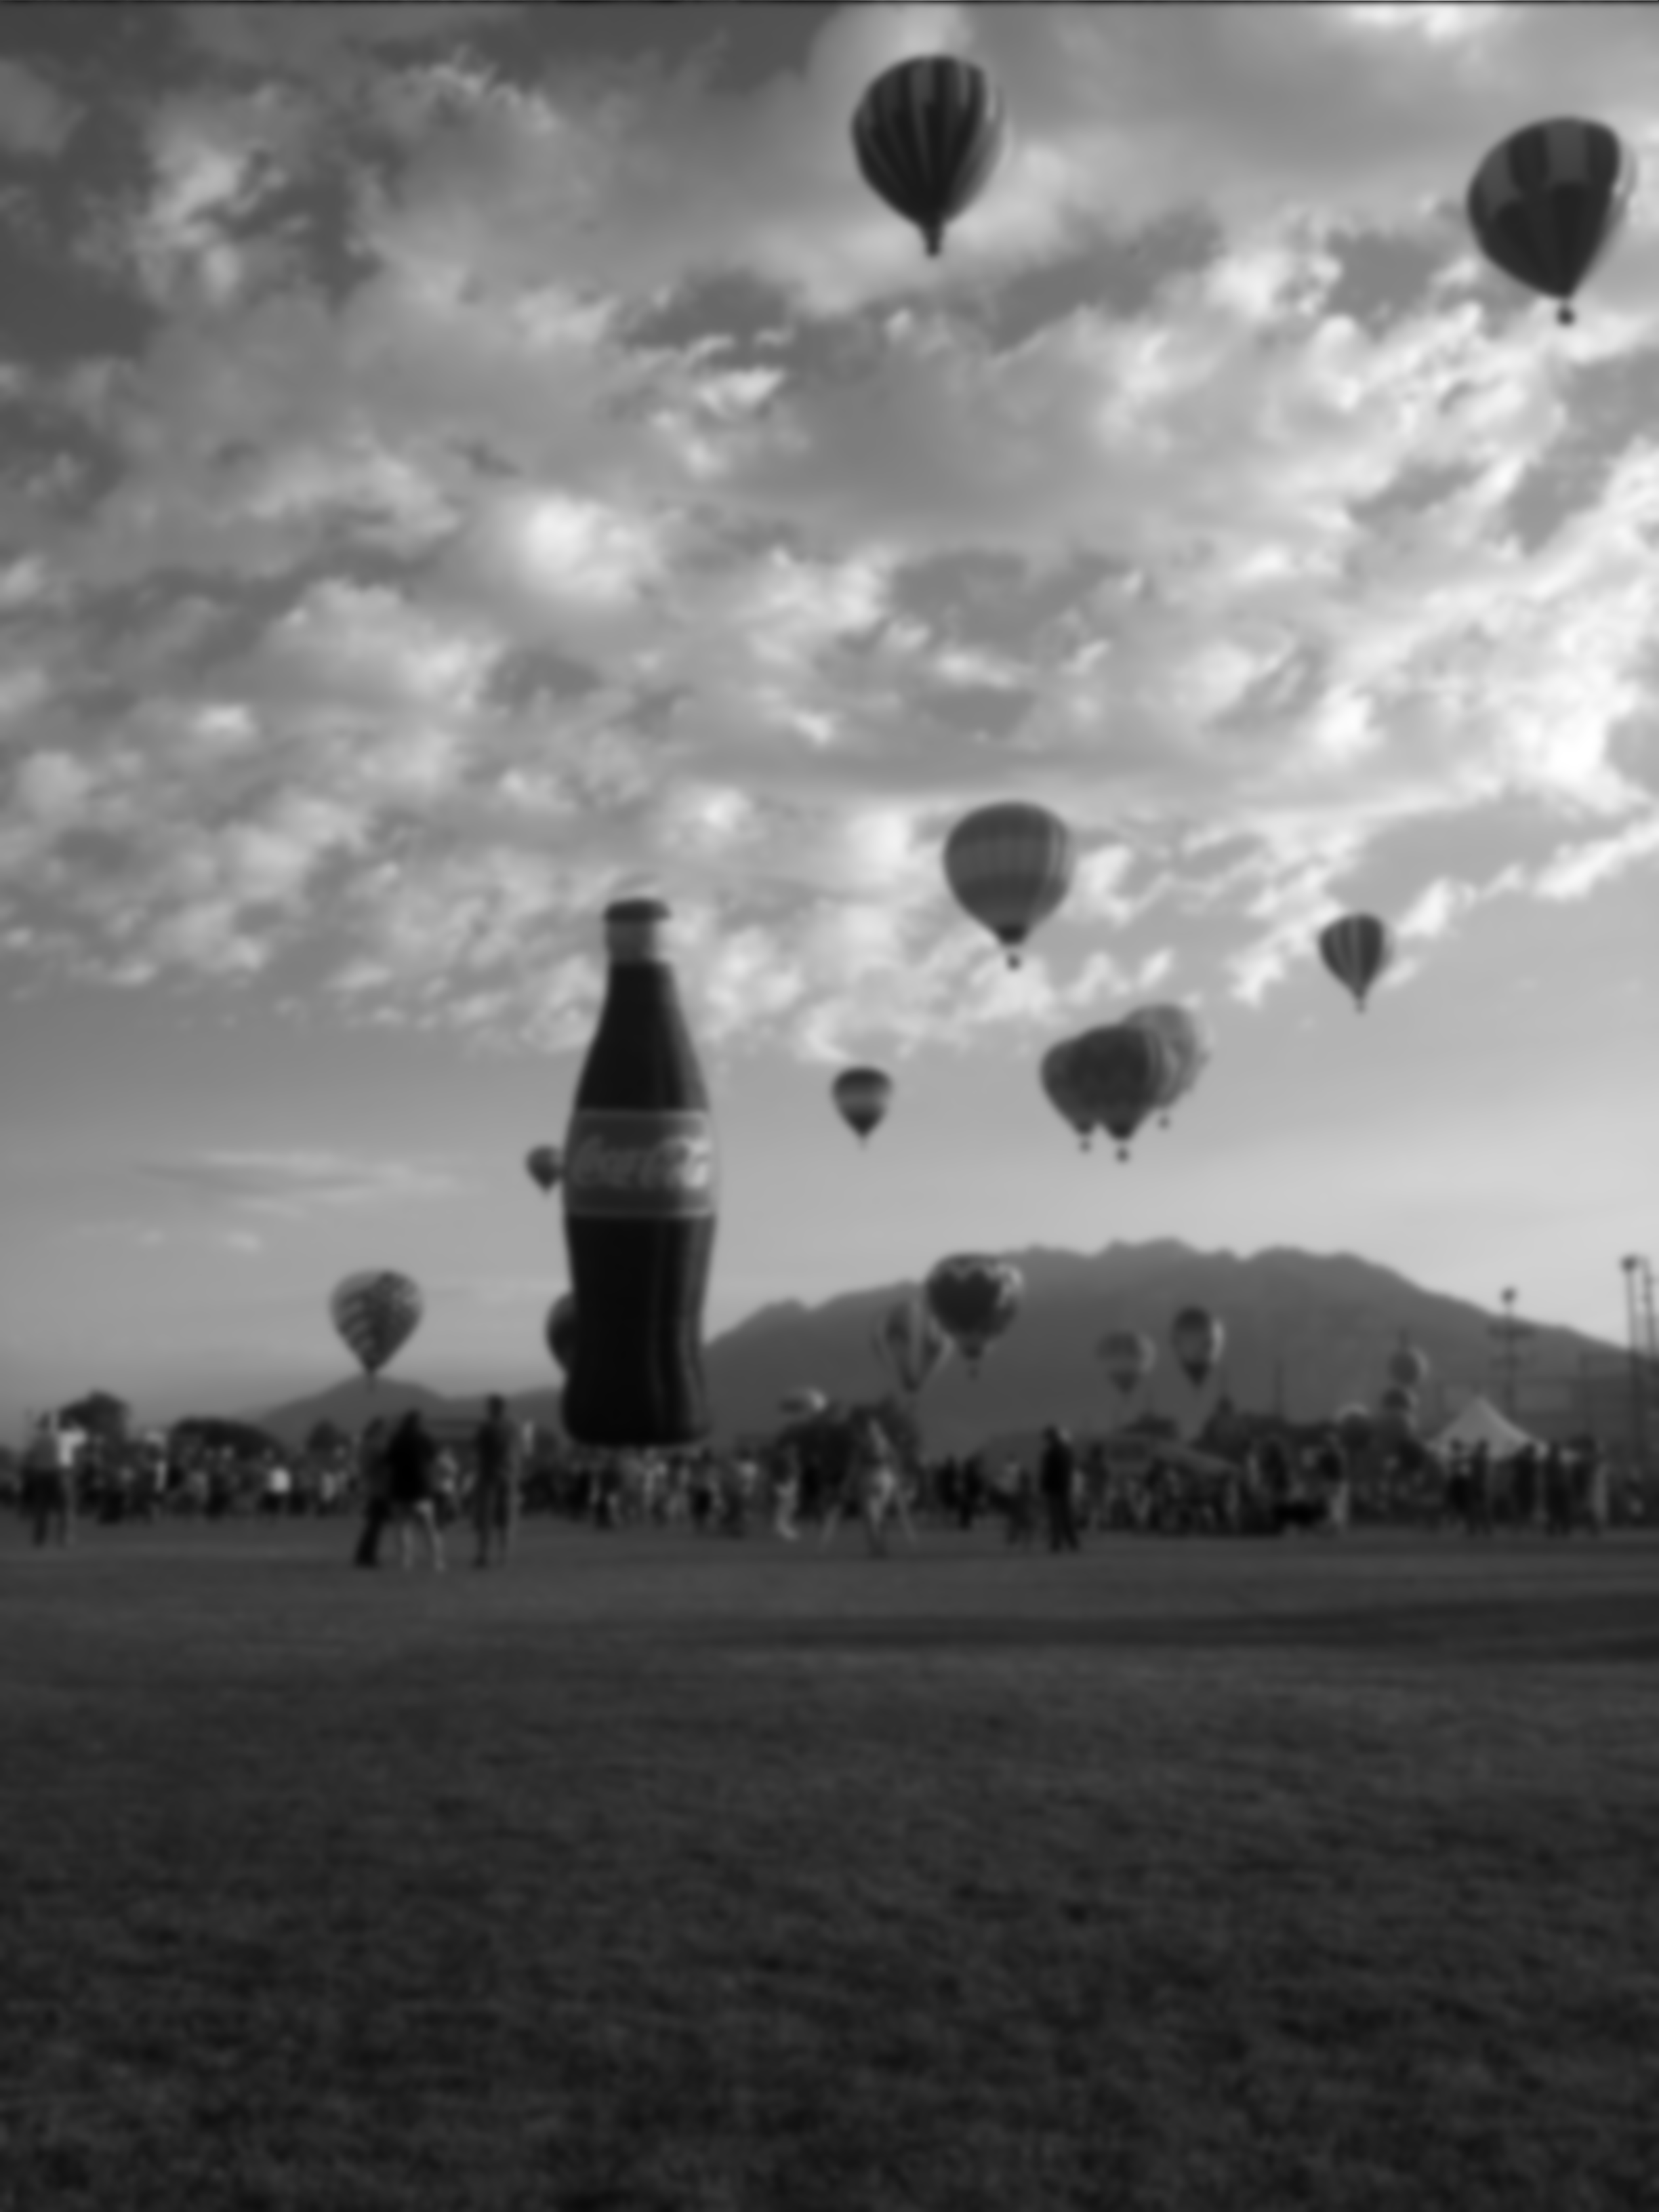
\includegraphics[width=\textwidth]{baloon100}
\caption*{after 100 iterations}
\end{minipage}
\hspace{0.5cm}
\begin{minipage}[b]{0.45\linewidth}
\centering
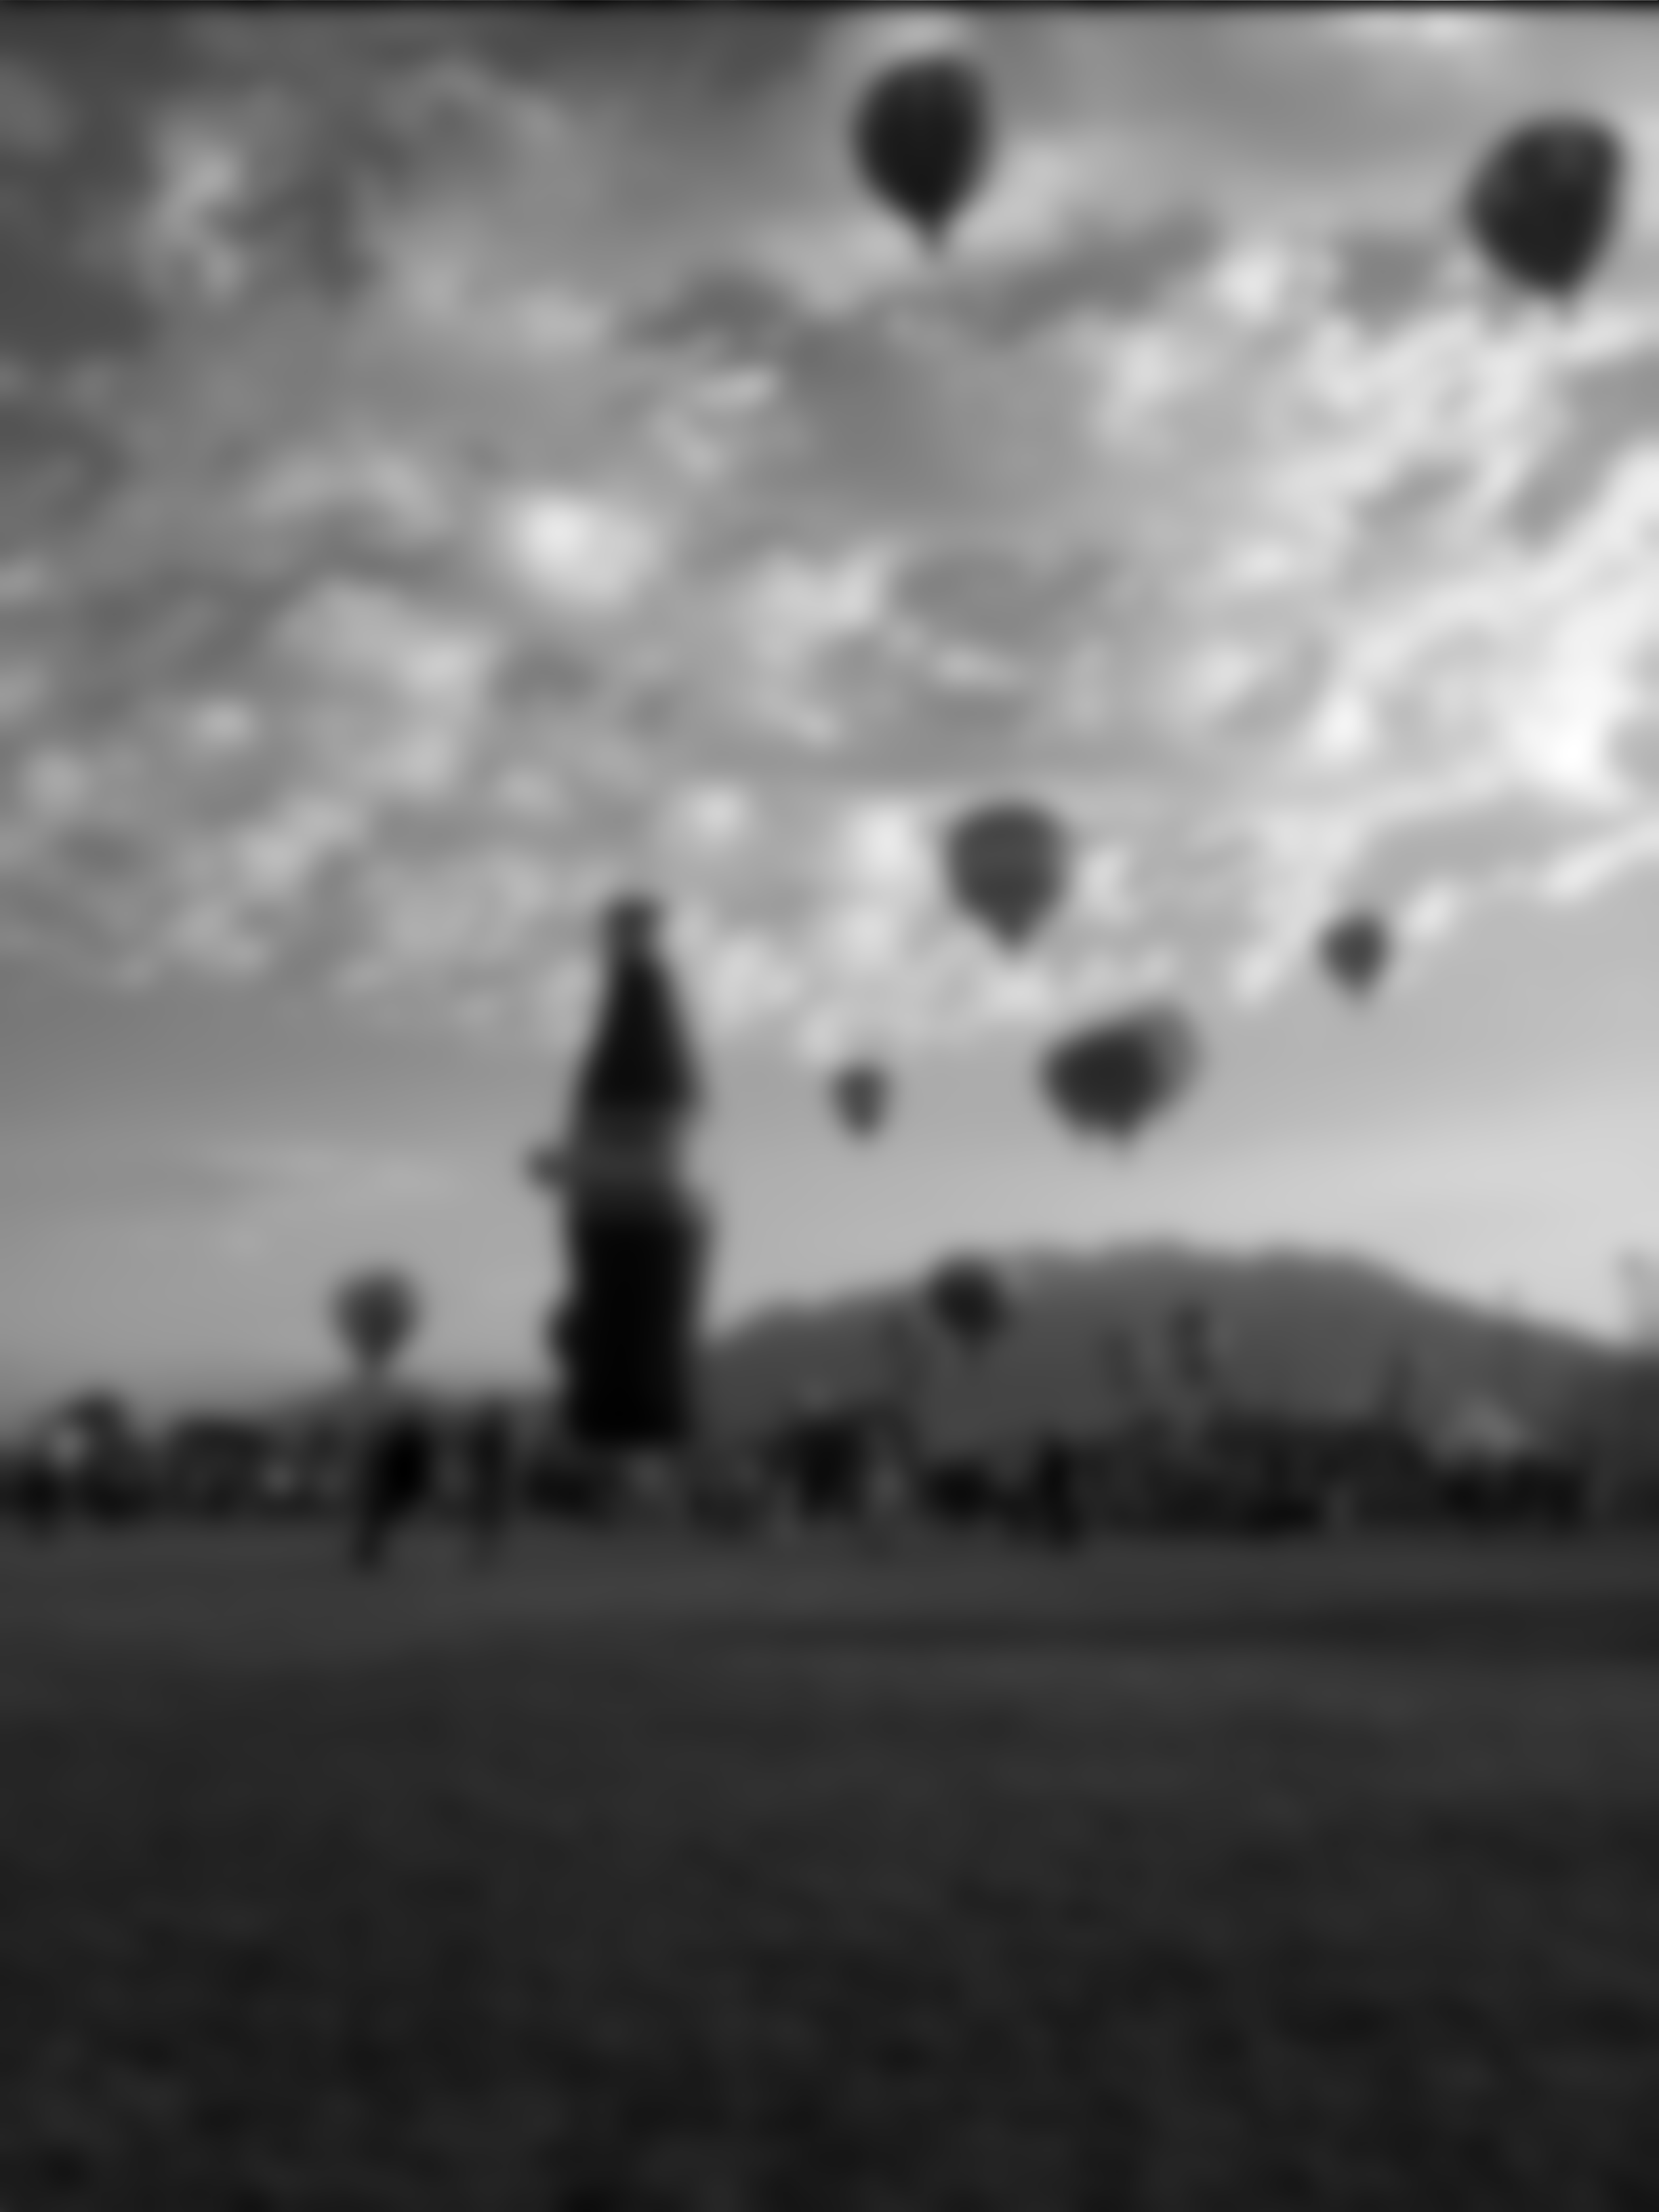
\includegraphics[width=\textwidth]{baloon1000}
\caption*{after 1000 iterations}
\end{minipage}
\end{figure}
\vfill
\clearpage

\begin{problem}
Implement the above finite difference scheme.
Leave the boundaries constant this time and just iterate over the interior of the image.
\end{problem}

\begin{problem}
Write a new version of the previous problem using the following boundary conditions:
For the top edge let 
\begin{equation*}
\begin{split}
v_{l,m}^{n+1} =& v_{l,m}^n + \lambda (g(|v_{l-1,m}^n - v_{l,m}|)(v_{l-1,m}^n - v_{l,m}) + g(|v_{l+1,m}^n - v_{l,m}|)(v_{l+1,m}^n - v_{l,m}) \\
 &+ g(|v_{l,m+1} - v_{l,m}|)(v_{l,m+1} - v_{l,m}))
\end{split}
\end{equation*}
Do the other edges similarly.

For the top left corner let
\begin{equation*}
v_{l,m}^{n+1} = v_{l,m}^n + \lambda (g(|v_{l+1,m}^n - v_{l,m}|)(v_{l+1,m}^n - v_{l,m}) + g(|v_{l,m+1} - v_{l,m}|)(v_{l,m+1} - v_{l,m}))
\end{equation*}
Do the other corners similarly.

Essentially we are just using the terms of the difference scheme that are actually defined.
\end{problem}

Colored images can be processed in a similar manner.
Instead of being represented as a two-dimensional array, colored images are represented as three dimensional arrays.
The third dimension is used to store the intensities of each of the standard 3 colors.
This diffusion process can be carried out in the exact same way, on each of the arrays of intensities for each color, but instead of detecting edges just in one color, we need to detect edges in any color, so instead of using something of the form $g(|v_{l+1,m}^n - v_{l,m}|)$ as before, we will now use something of the form $g(||v_{l+1,m}^n - v_{l,m}||)$, where $v_{l+1,m}^n$ and $v_{l,m}$ are vectors now instead of scalars.
The difference scheme can be treated as an eqation on vectors in 3-space and now reads:
\begin{equation*}
\begin{split}
v_{l,m}^{n+1} =& v_{l,m}^n + \lambda (g(||v_{l-1,m}^n - v_{l,m}||)(v_{l-1,m}^n - v_{l,m}) + g(||v_{l+1,m}^n - v_{l,m}||)(v_{l+1,m}^n - v_{l,m}) \\
 &+ g(||v_{l,m-1} - v_{l,m}||)(v_{l,m-1} - v_{l,m}) + g(||v_{l,m+1} - v_{l,m}||)(v_{l,m+1} - v_{l,m}))
\end{split}
\end{equation*}

\newpage
\vfill
\begin{figure}[ht]
\begin{minipage}[b]{0.45\linewidth}
\centering
\includegraphics[width=\textwidth]{baloon_col}
\caption*{original image}
\end{minipage}
\hspace{0.5cm}
\begin{minipage}[b]{0.45\linewidth}
\centering
\includegraphics[width=\textwidth]{baloon_col20}
\caption*{after 20 iterations with $\sigma = .7$ and $\lambda = .2$}
\end{minipage}
\begin{minipage}[b]{0.45\linewidth}
\centering
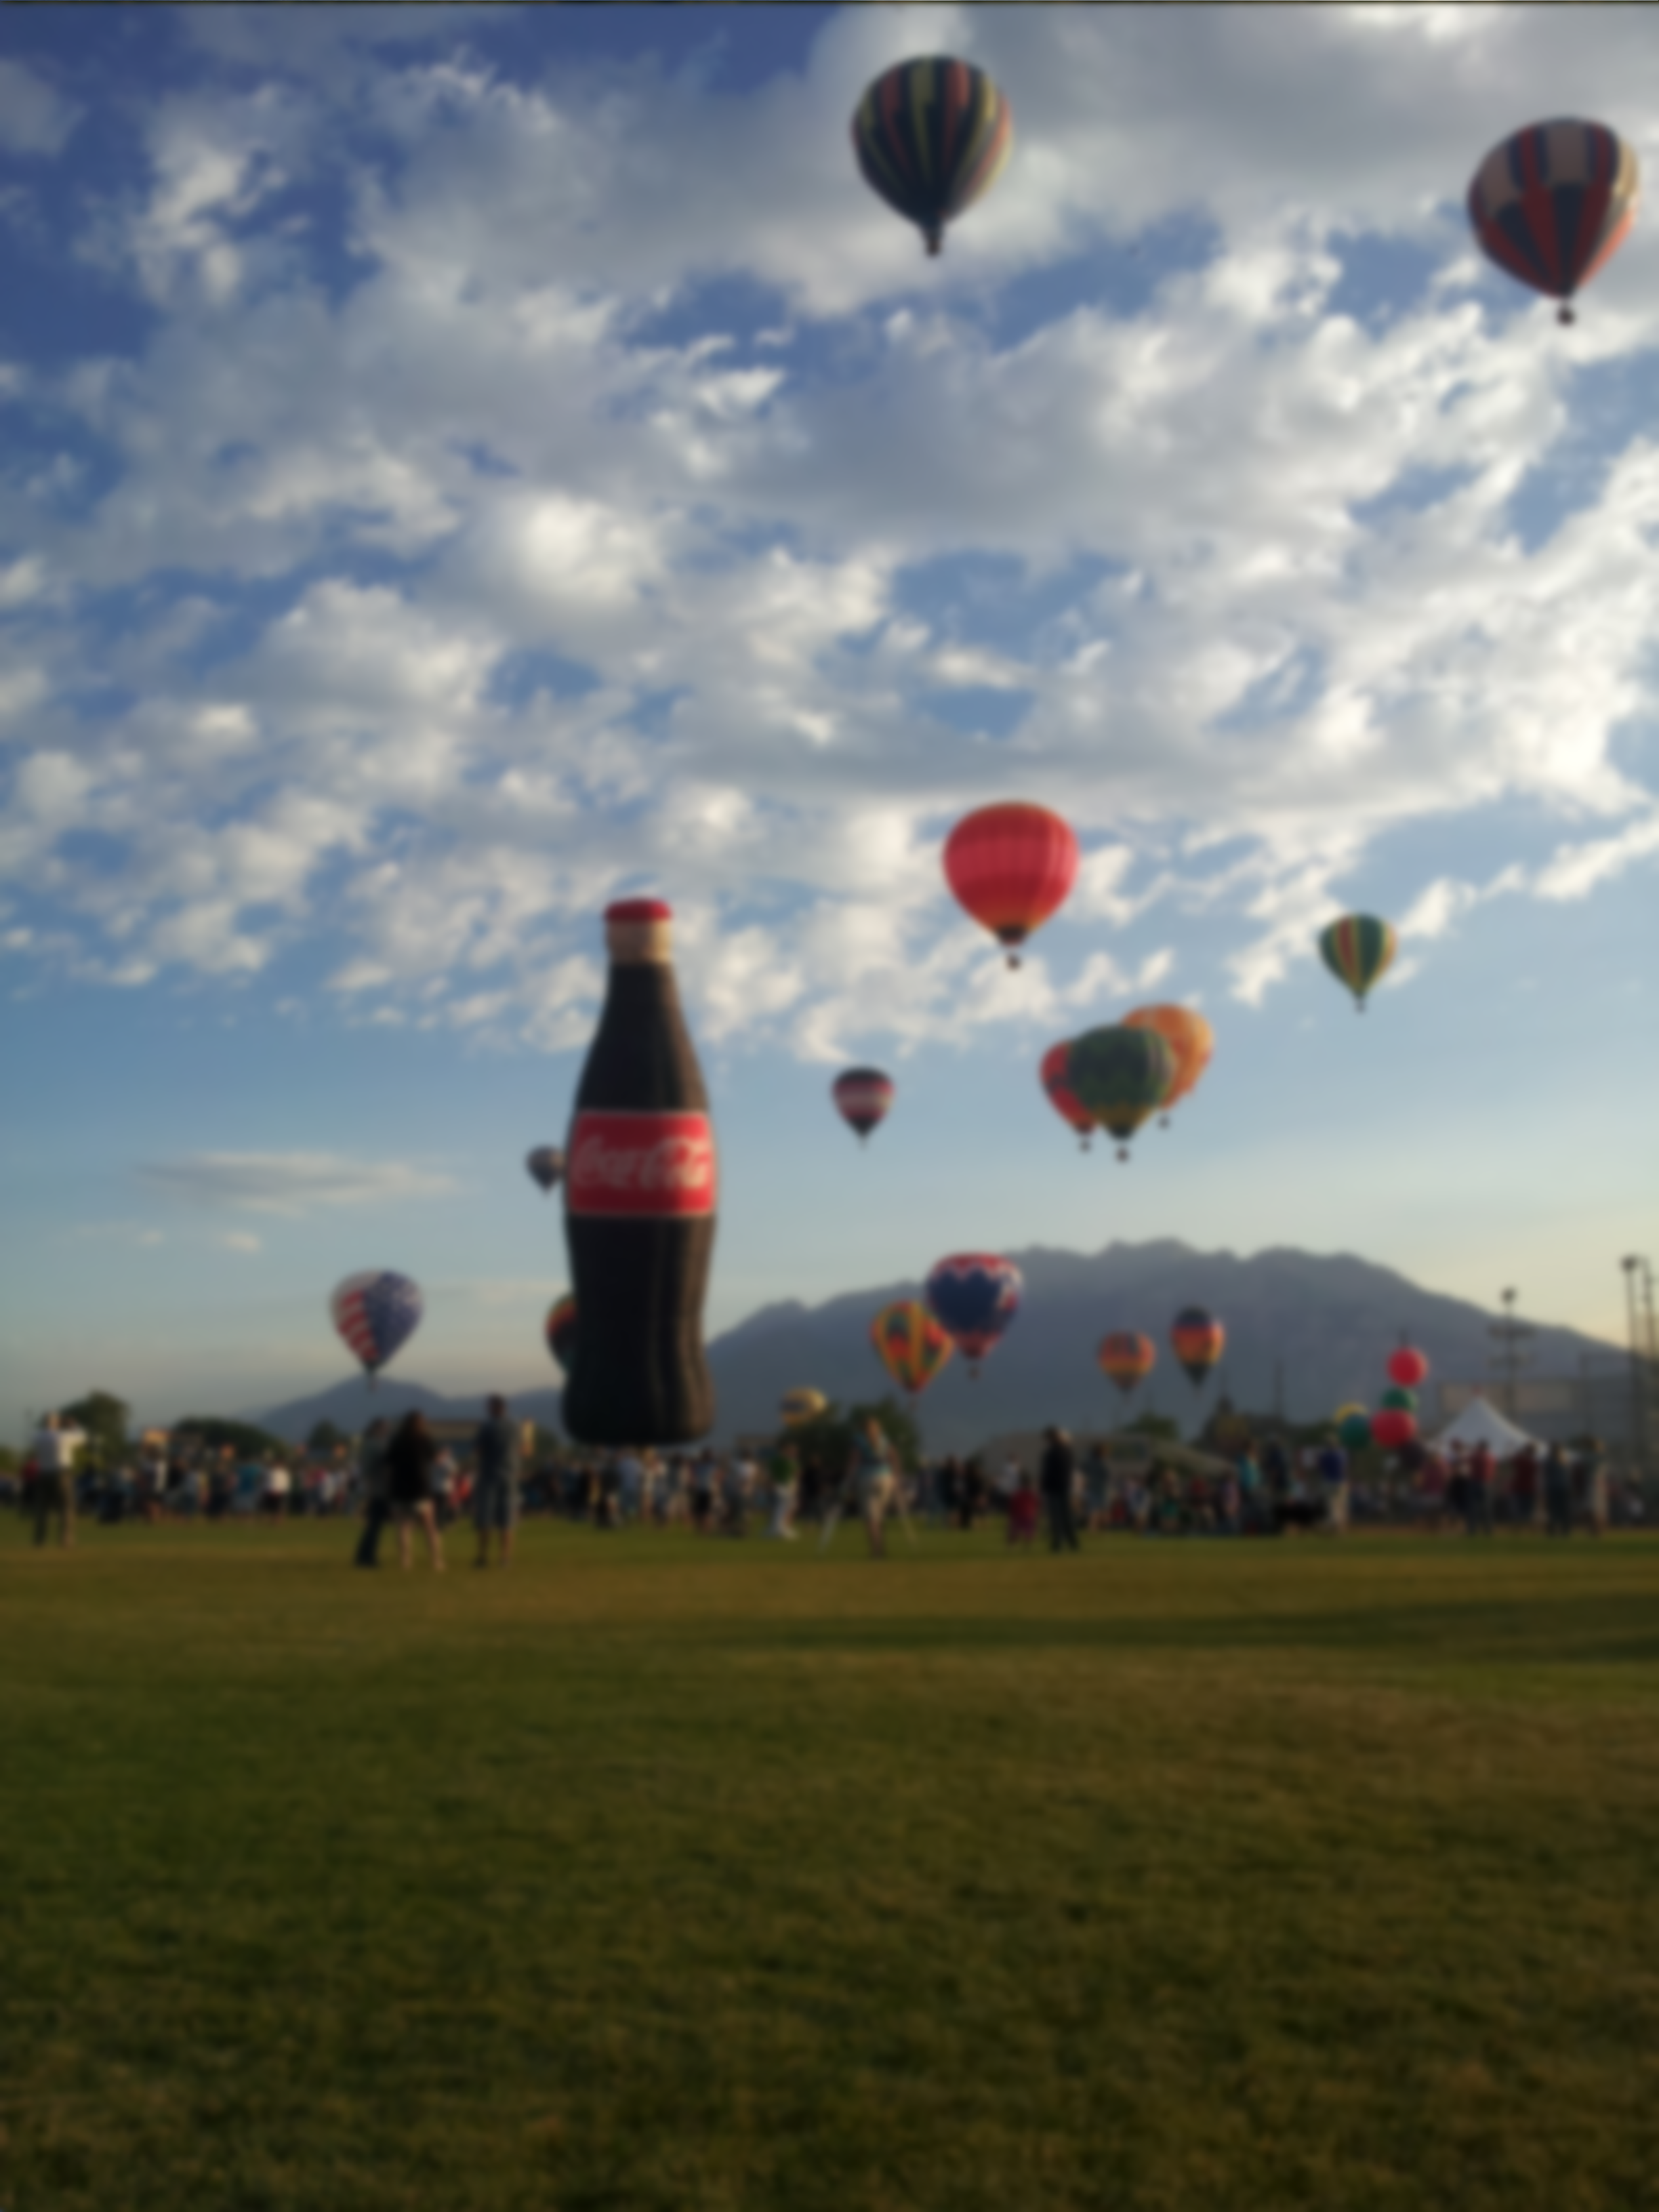
\includegraphics[width=\textwidth]{baloon_col100}
\caption*{after 100 iterations}
\end{minipage}
\hspace{0.5cm}
\begin{minipage}[b]{0.45\linewidth}
\centering
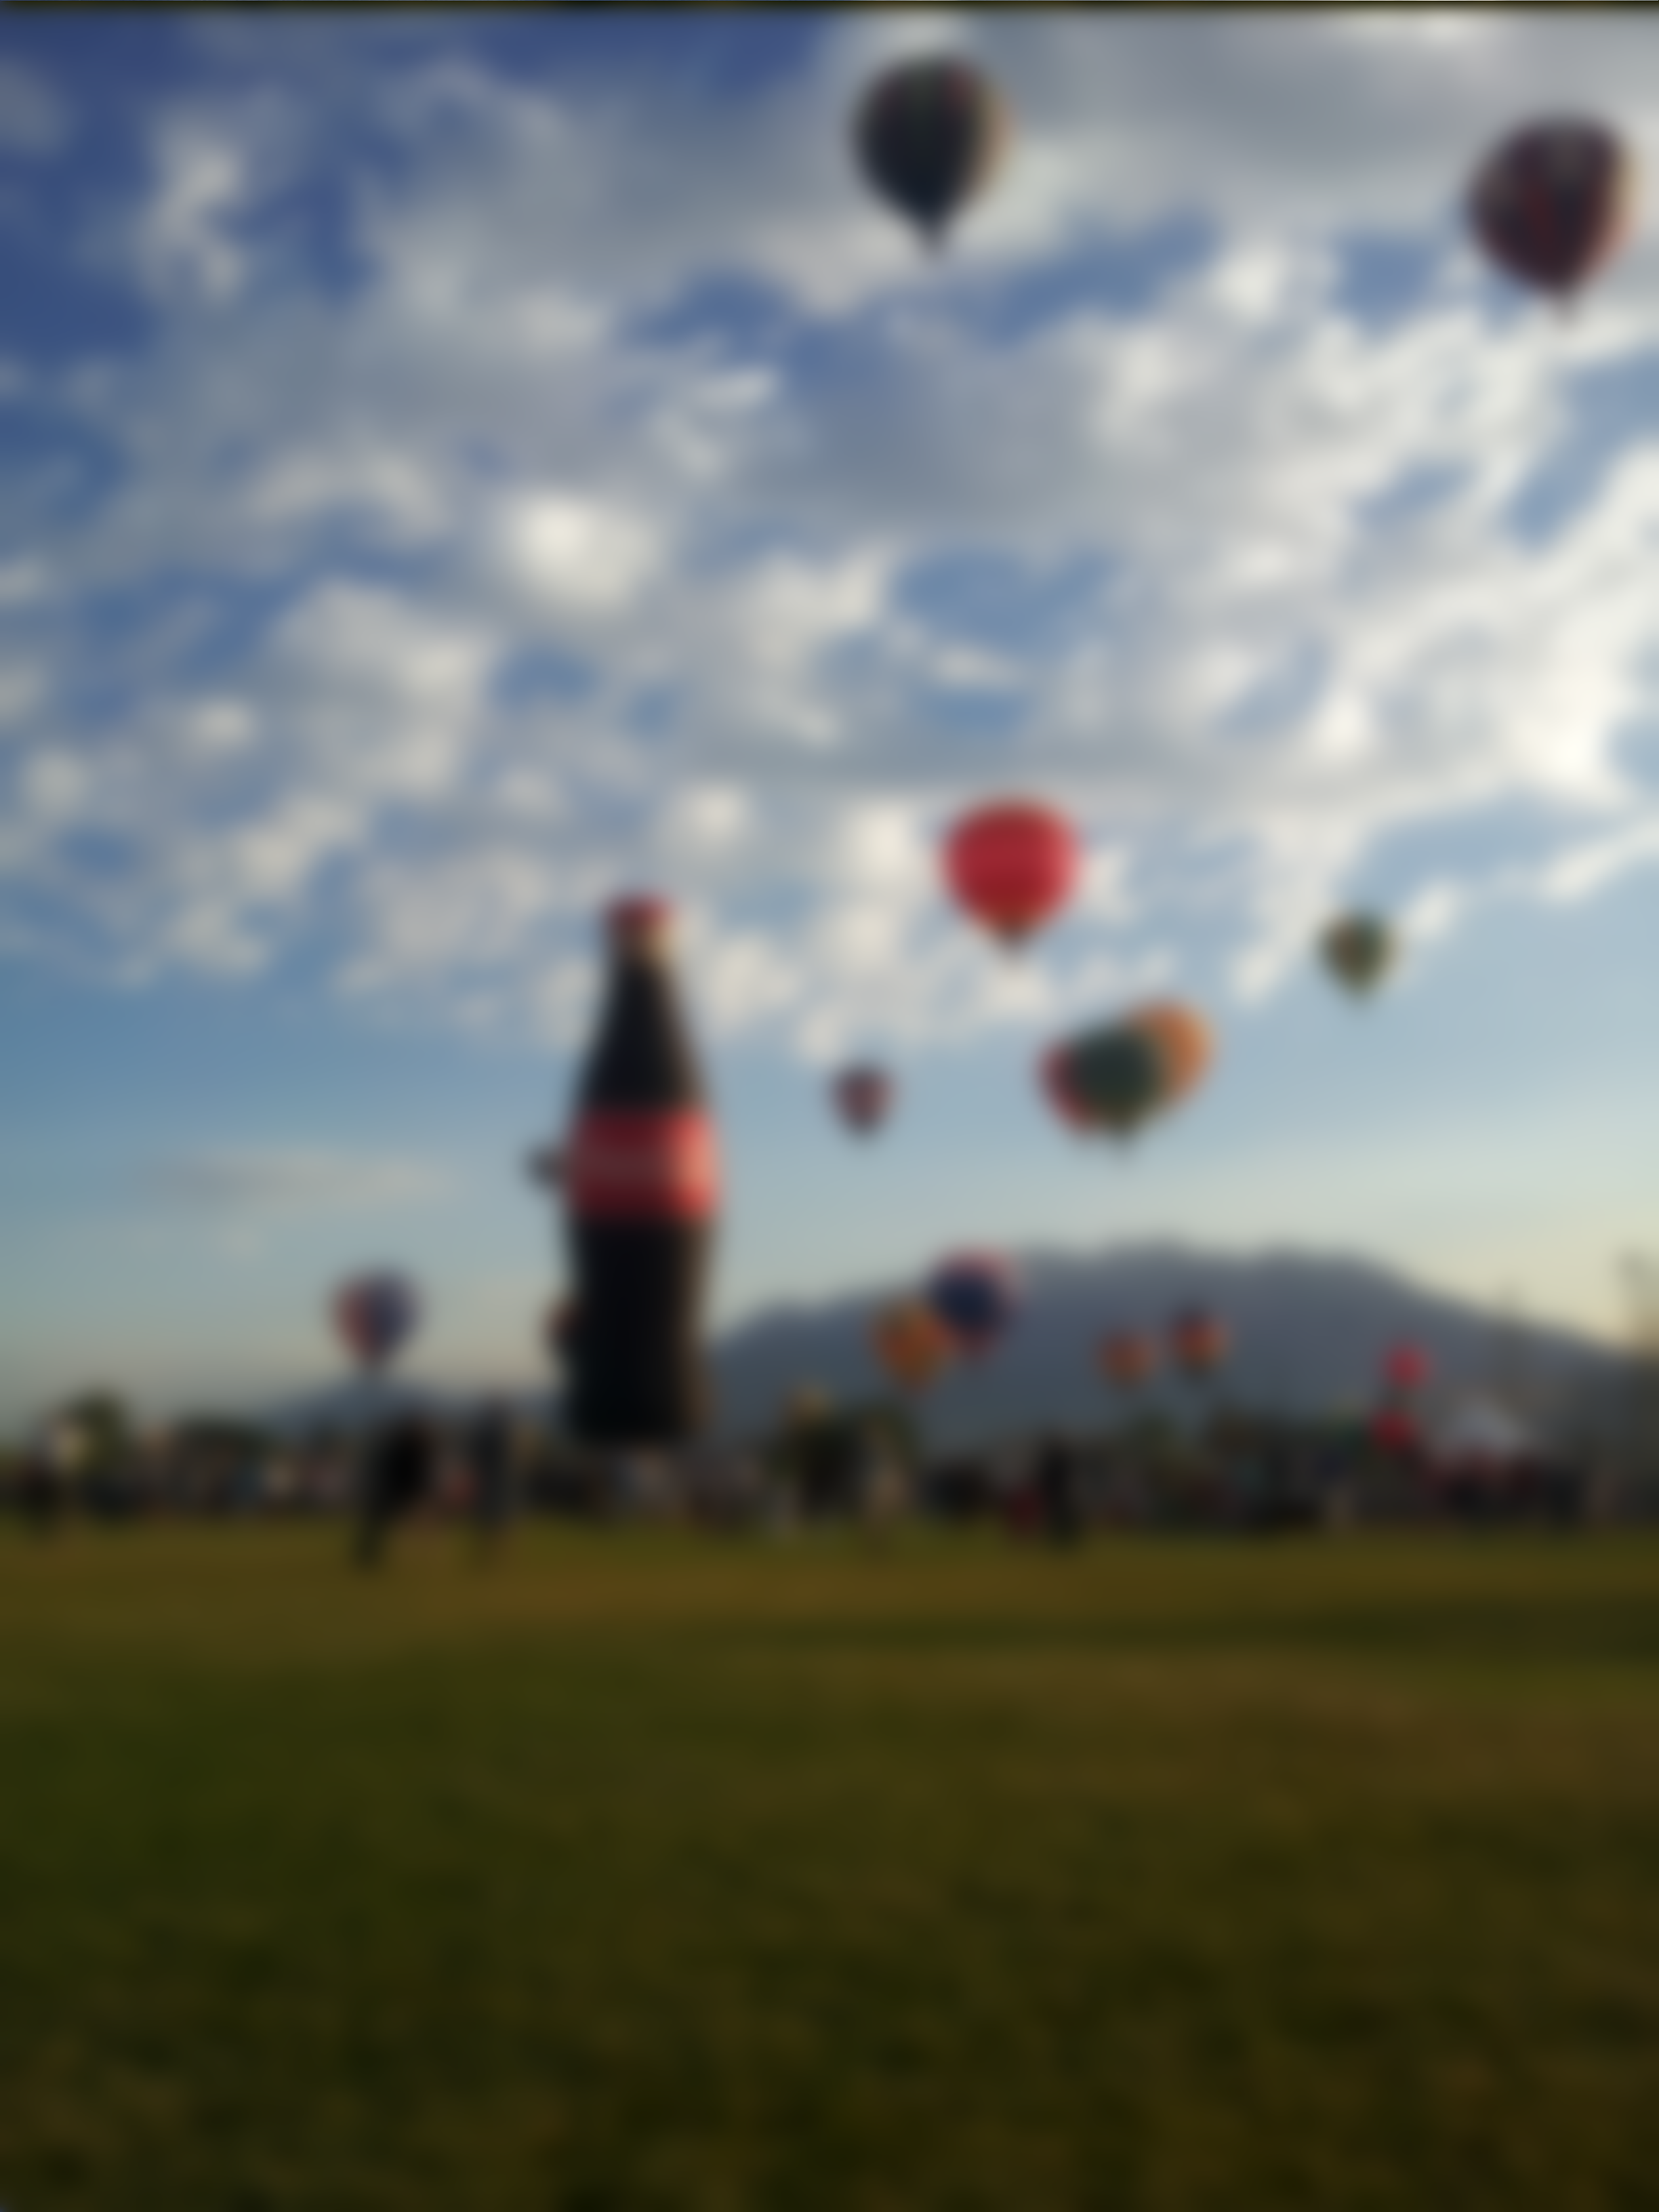
\includegraphics[width=\textwidth]{baloon_col1000}
\caption*{after 1000 iterations}
\end{minipage}
\end{figure}
\vfill
\clearpage

\begin{problem}
Make a new version of the code you wrote for the previous problem which processes a colored image.
\end{problem}

This sort of anisotropic diffusion can be very effective, but, depending on the image, it may also smear out edges that do not have large gradients between them.
A similar way of denoising the image involves limiting the influence of diffusion on points that are adjacent to points of similar value.
This will quickly remove isolated pixels that are dissimilar from their surroundings, but it may not allow the image to change as much under so many iterations.

An example of this can be seen in the following image.
The following are the original image and the filtered images after 20, and 100 iterations.
In this case we used $\sigma = .1$ and $\lambda = .25$

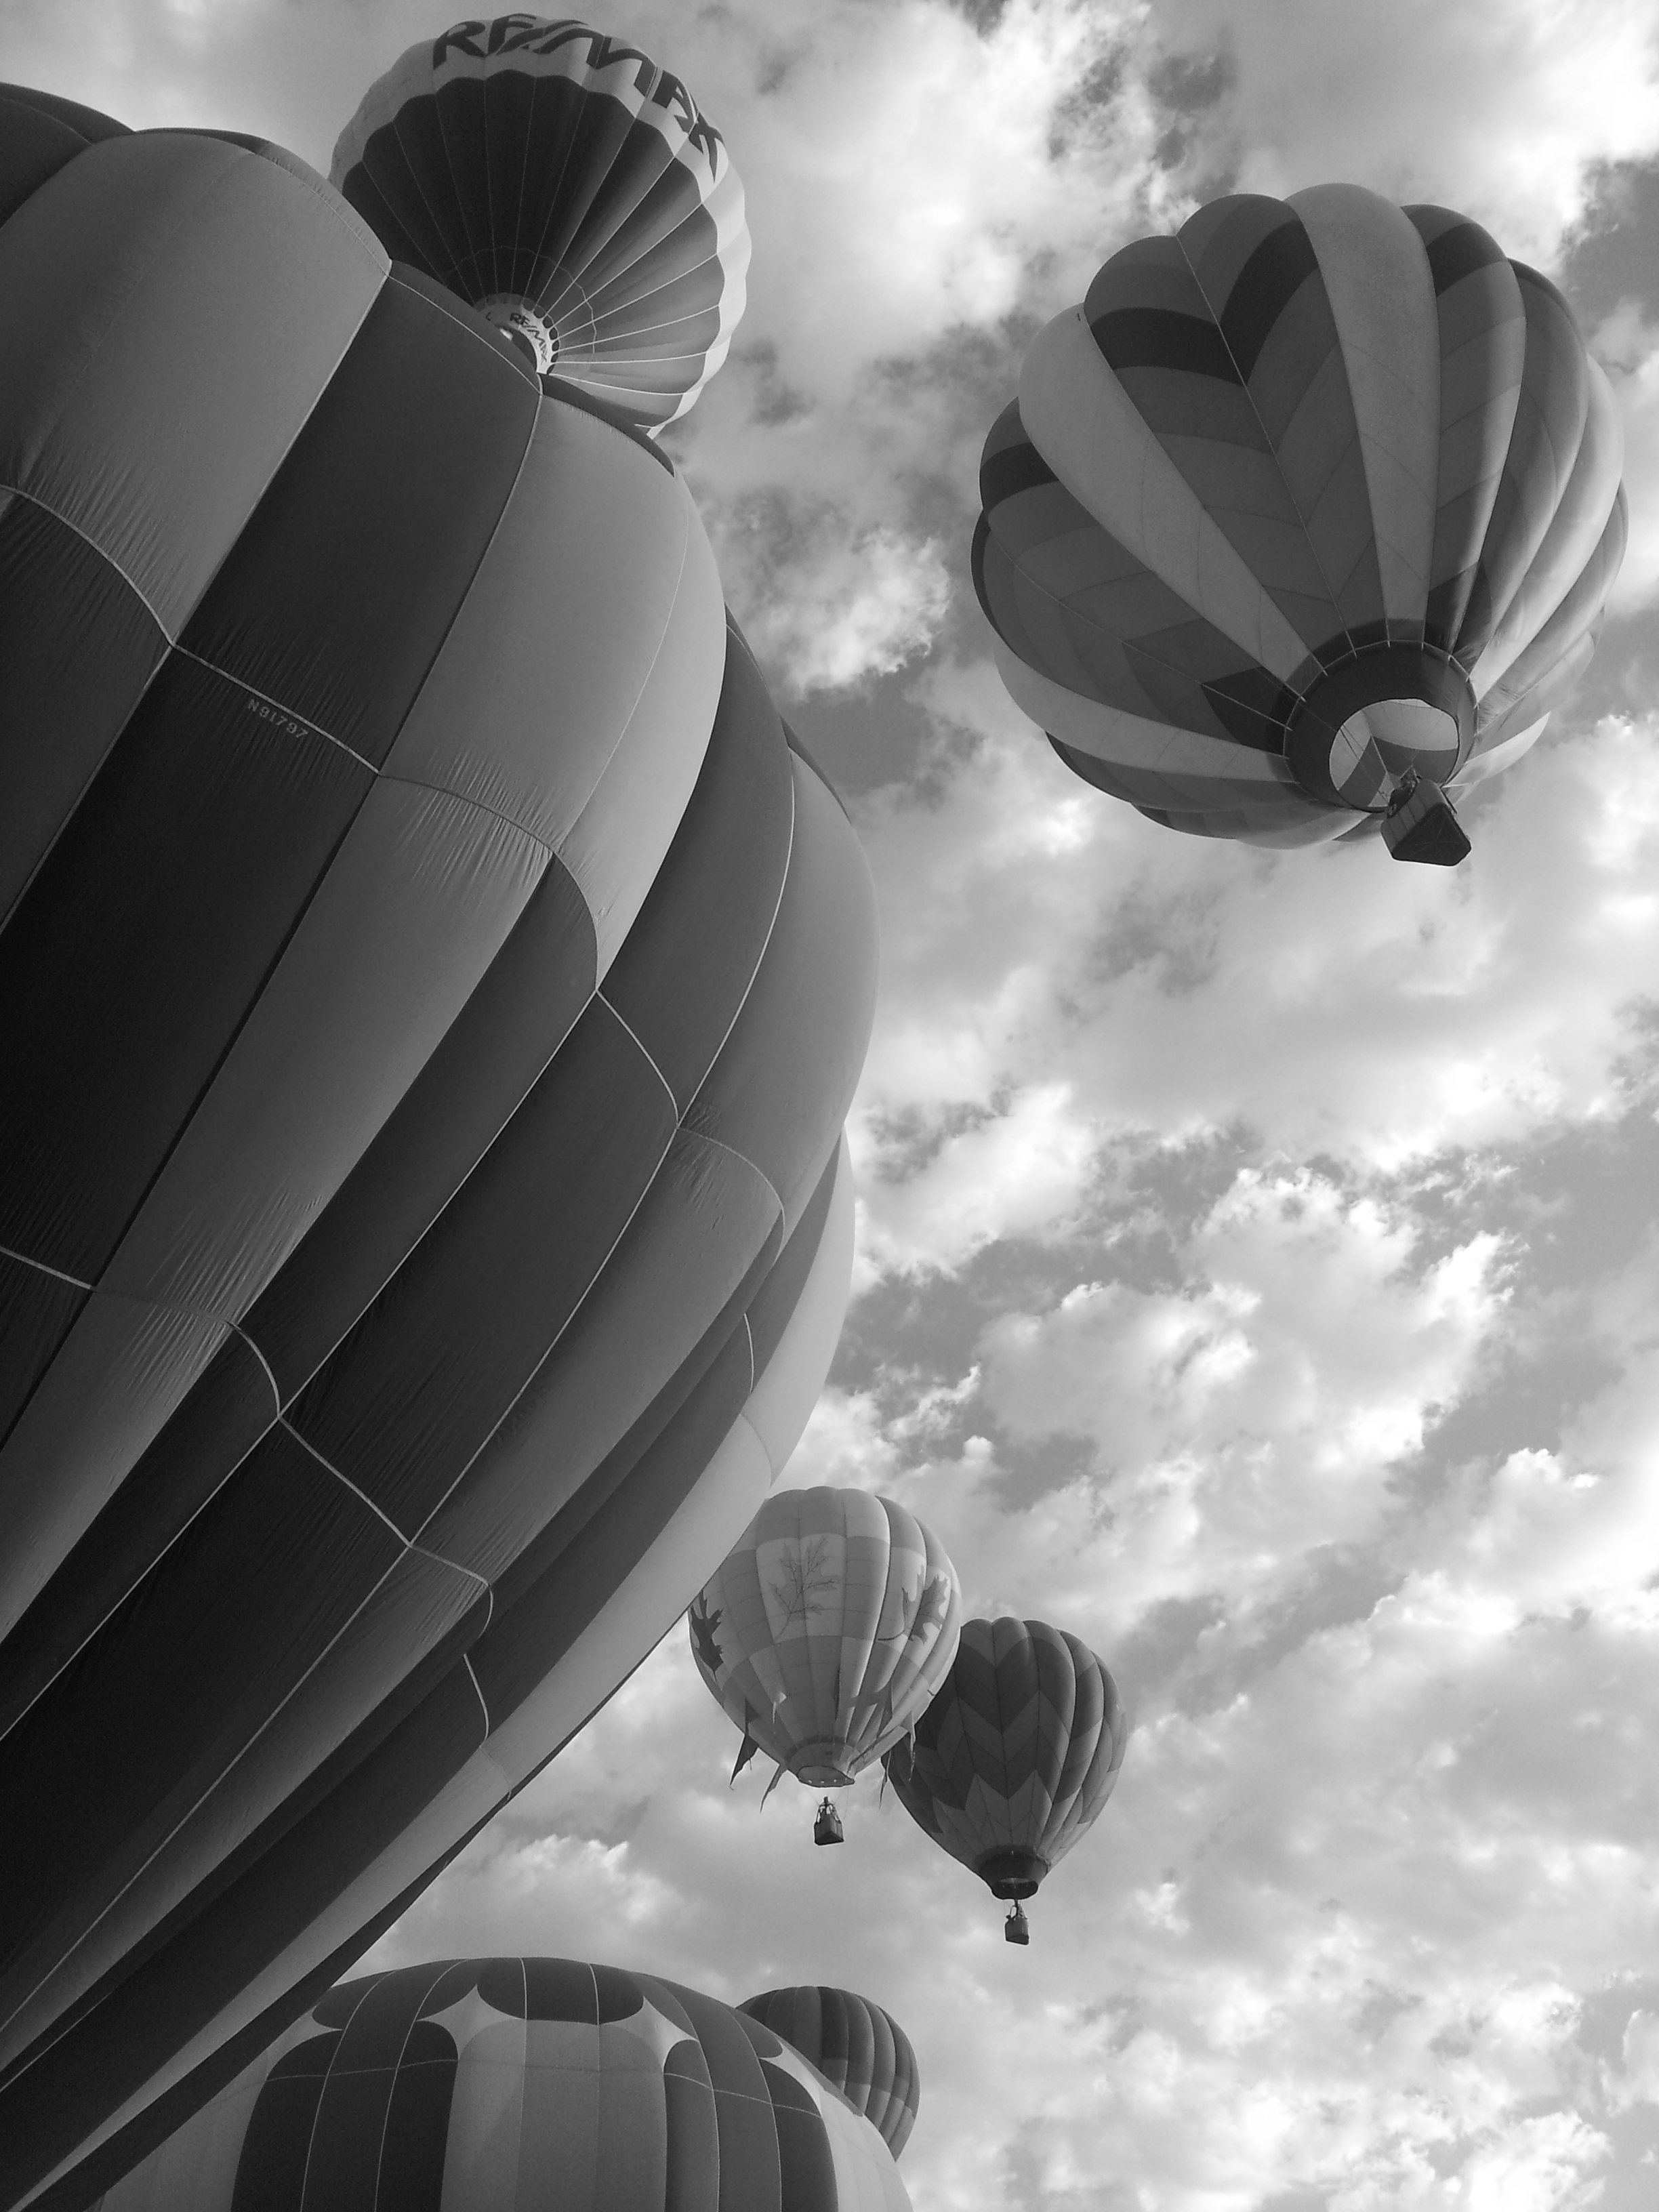
\includegraphics[width=\textwidth]{baloonsbw}

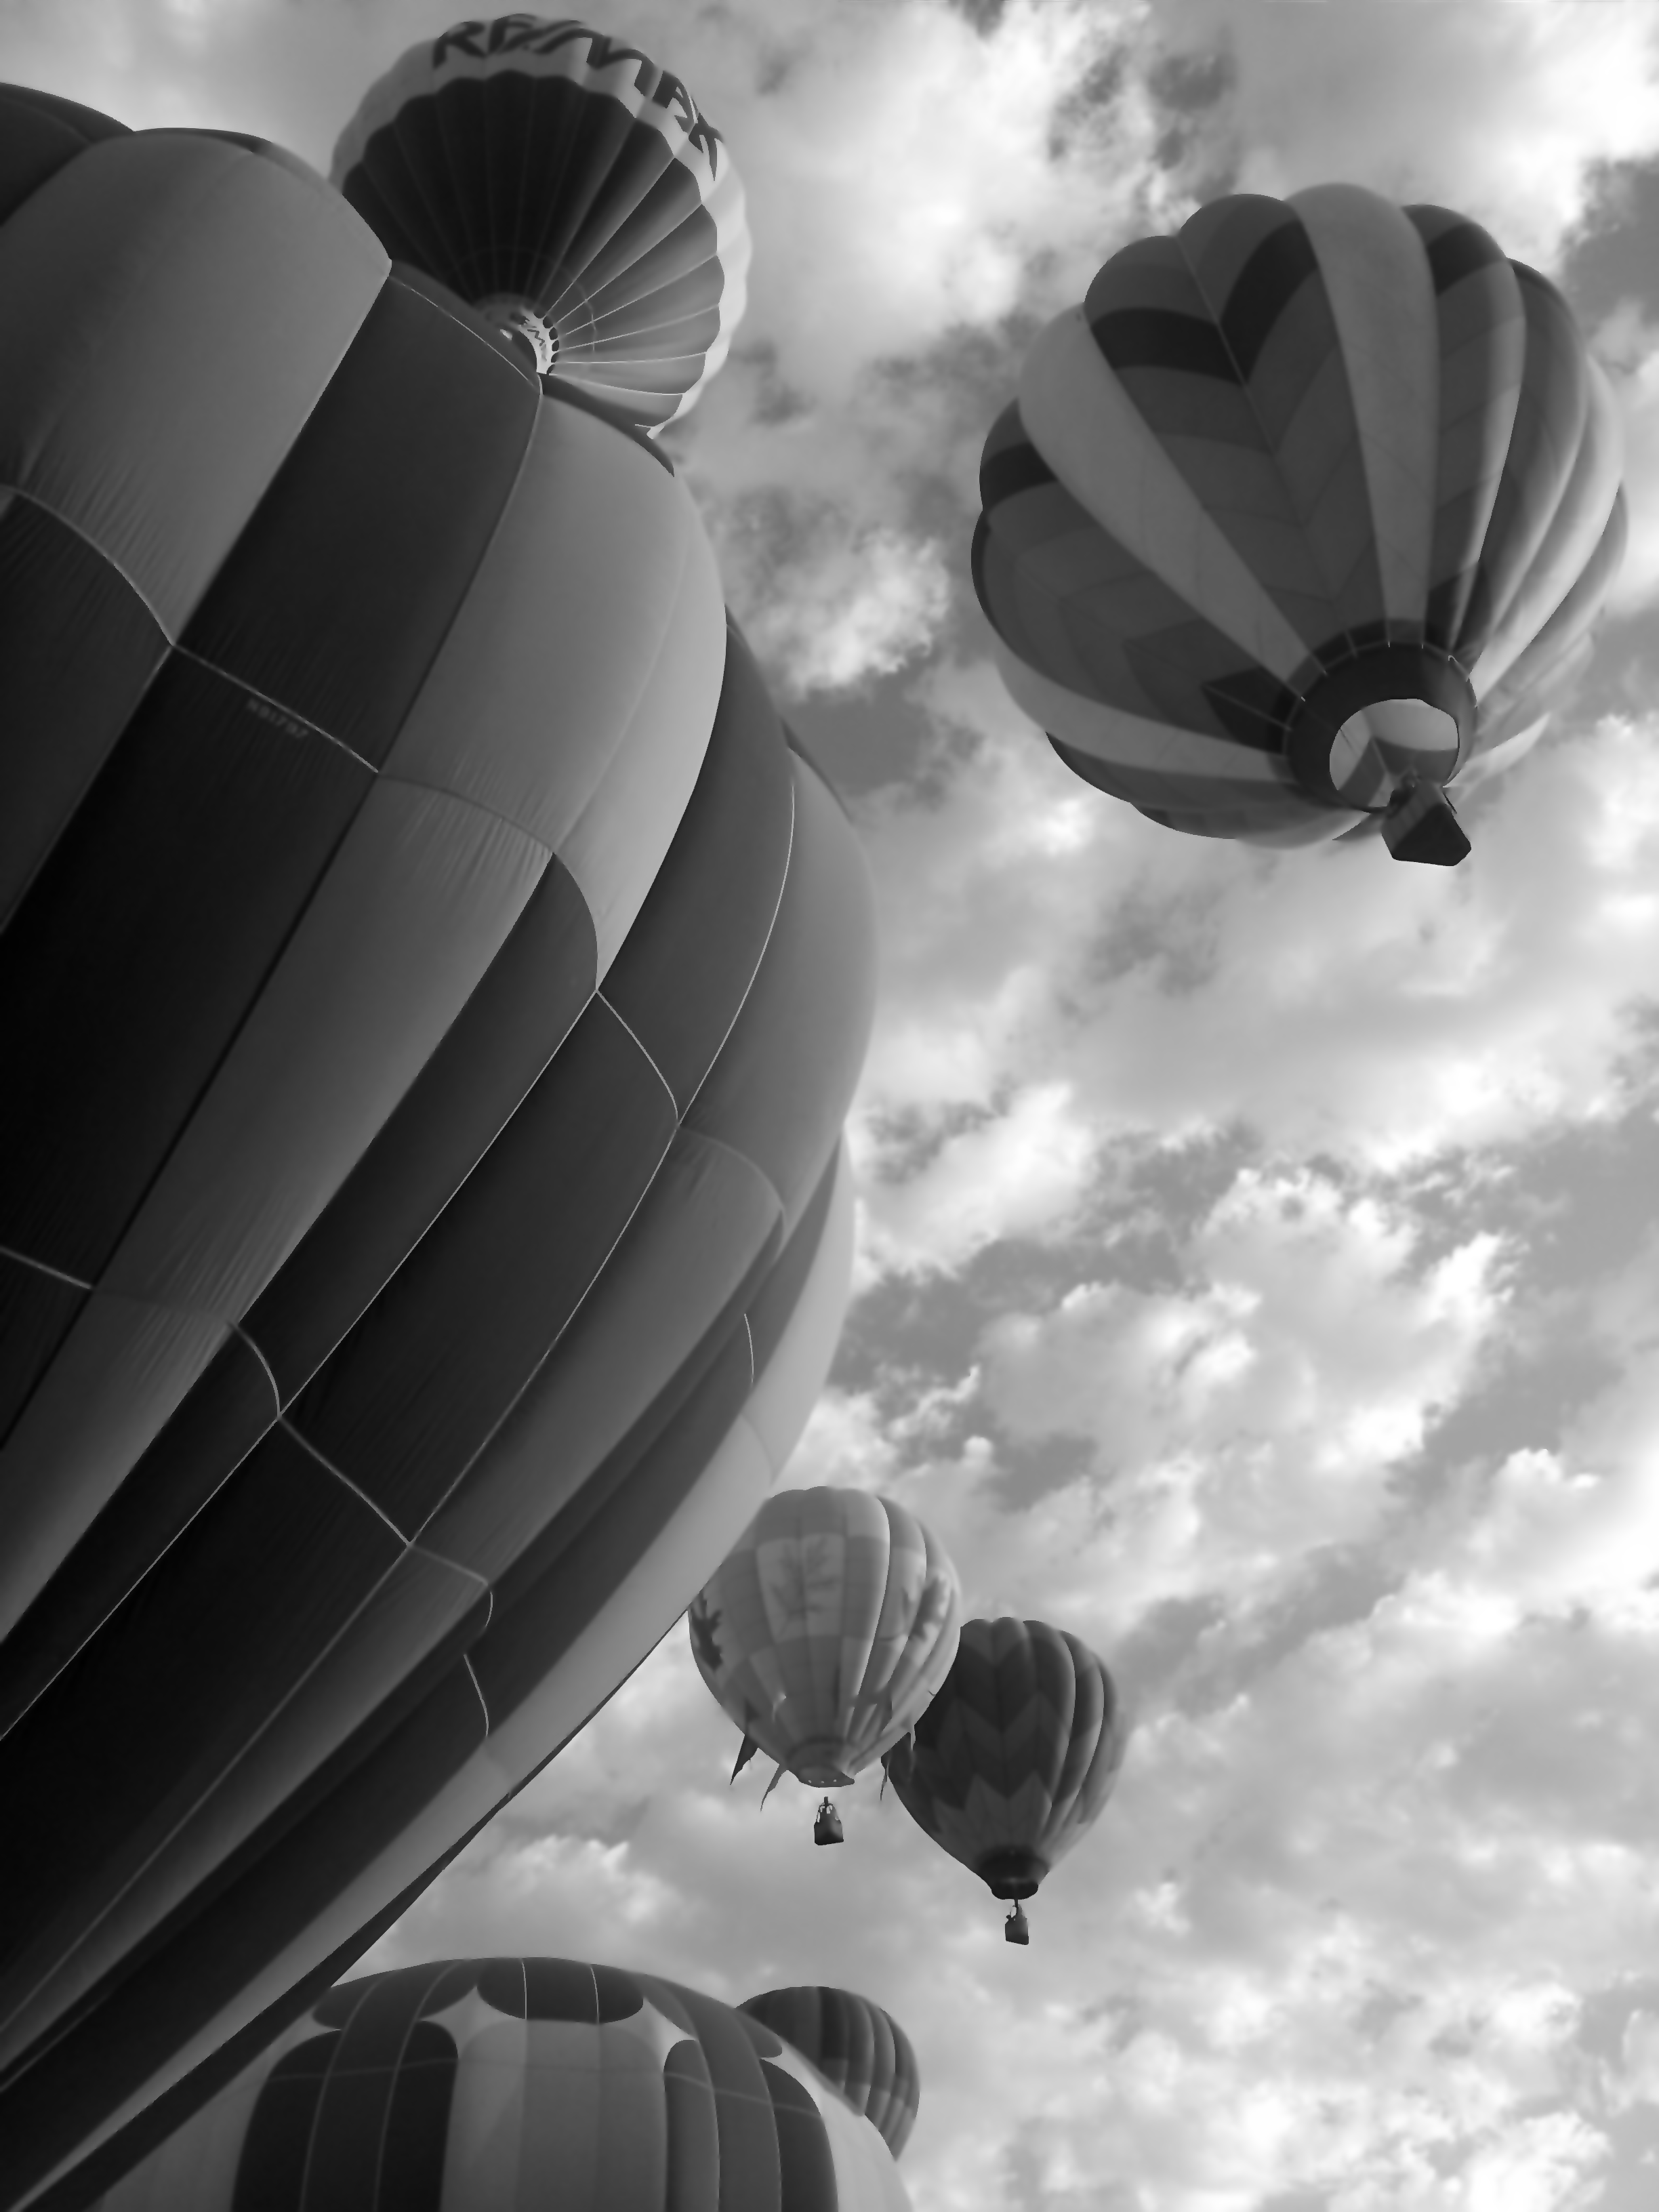
\includegraphics[width=\textwidth]{baloons20}

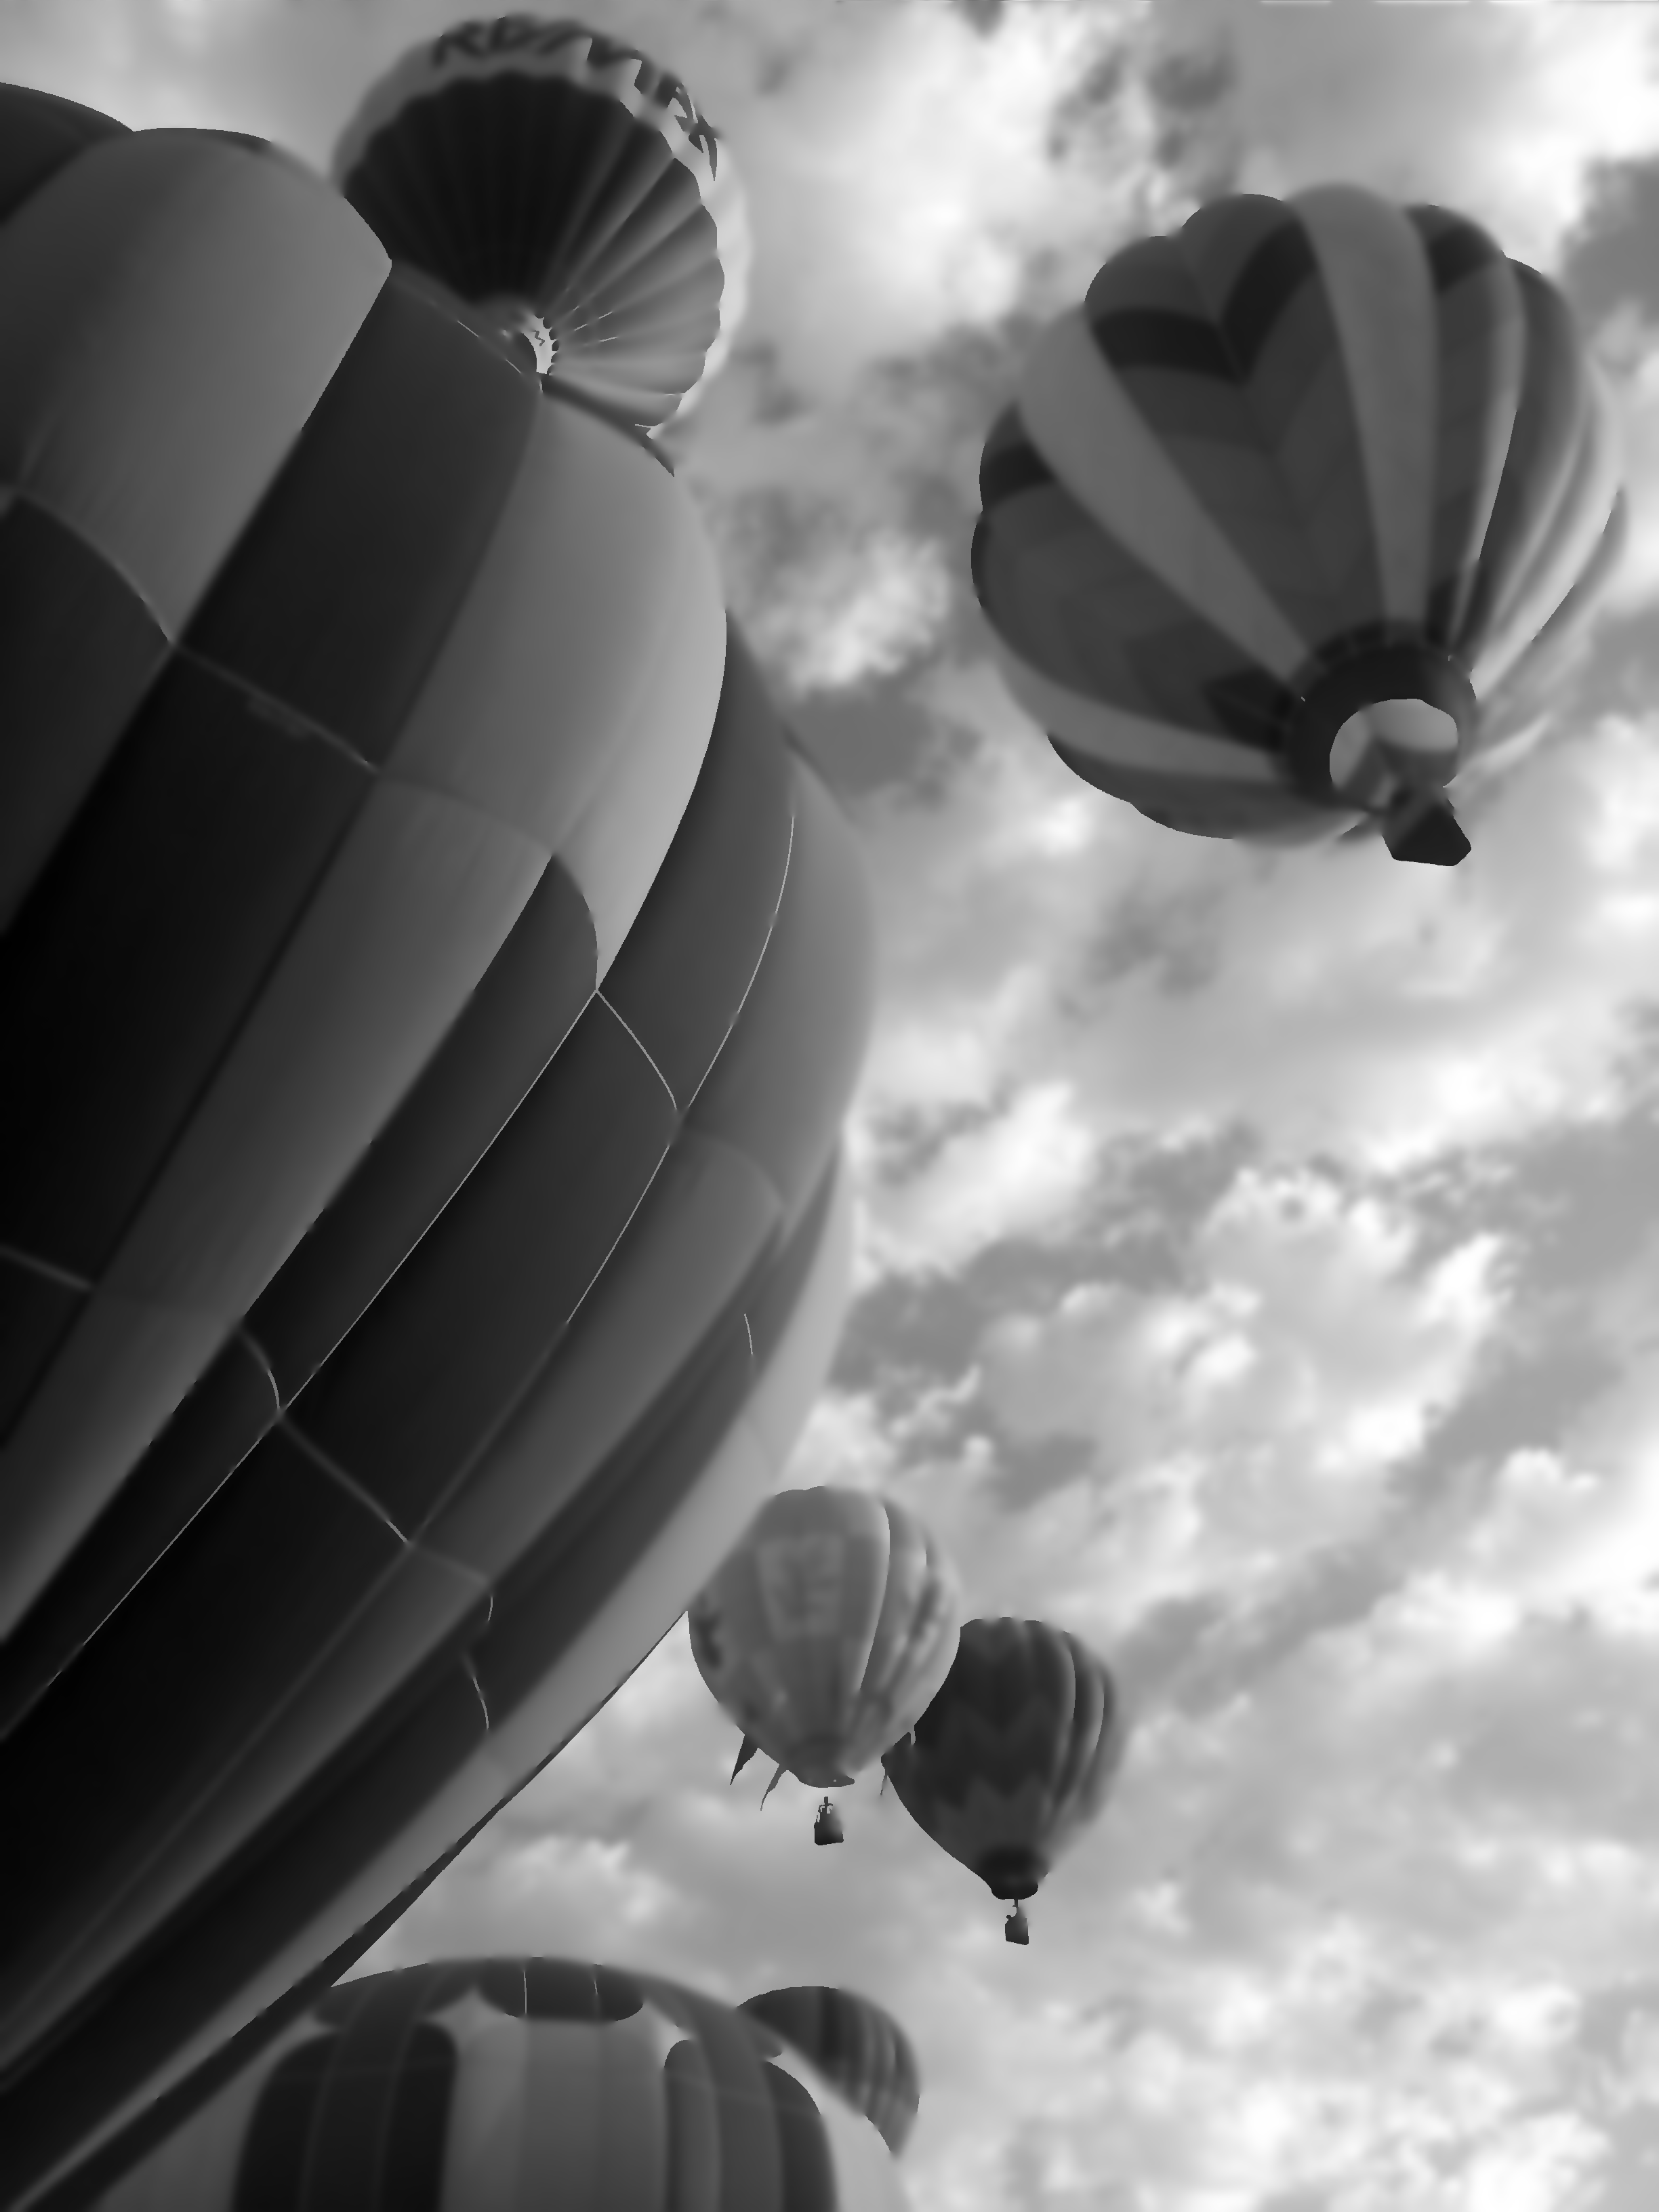
\includegraphics[width=\textwidth]{baloons100}

As we can see, after 100 iterations, some of the boundaries between similar shades of grey have smeared unevenly.